% TO-DO:
% * fuzzy logic re-write
% * classifying spaces *
% * Yoneda lemma finish
% * functorial semantics
% * Kripke-Joyal semantics
% * Cohen forcing *
% * Sheaves and topos *
% * Heyting algebra revise *

% * implementation of topology ***
% * model-based approach

% DONE:
% * The model is only for working memory.  
% * Even so, what does the model offer that syntax does not have?
% * Need a simple semantic model to begin thinking....

\input{../YKY-preamble.tex}

\usepackage{color}
\usepackage{mathtools}
\usepackage{hyperref}

\usepackage[backend=biber,style=numeric]{biblatex}
\bibliography{../AGI-book}
% \renewcommand*{\bibfont}{\footnotesize}

\usepackage{graphicx} % Allows including images
\usepackage{tikz-cd}
\usepackage{tikz}
\usepackage[export]{adjustbox}% http://ctan.org/pkg/adjustbox
\usepackage{verbatim} % for comments
% \usepackage{newtxtext,newtxmath}	% Times New Roman font

\numberwithin{equation}{subsection}

\newcommand{\underdash}[1]{%
	\tikz[baseline=(toUnderline.base)]{
		\node[inner sep=1pt,outer sep=10pt] (toUnderline) {#1};
		\draw[dashed] ([yshift=-0pt]toUnderline.south west) -- ([yshift=-0pt]toUnderline.south east);
	}%
}%

\DeclareSymbolFont{symbolsC}{U}{txsyc}{m}{n}
\DeclareMathSymbol{\strictif}{\mathrel}{symbolsC}{74}

\newcommand{\highlight}[1]{\colorbox{pink}{$\displaystyle #1$}}

\newcommand{\emp}[1]{{\color{violet}\textbf{#1}}}
\newcommand*\confoundFace{$\vcenter{\hbox{\includegraphics[scale=0.2]{../2020/../confounded-face.jpg}}}$}
\newcommand{\underconst}{\includegraphics[scale=0.5]{../2020/UnderConst.png}}
\newcommand{\witness}{\scalebox{0.6}{$\blacksquare$}}
% \newcommand{\Heytingarrow}{\mathrel{-}\mathrel{\triangleright}}
\providecommand\Heytingarrow{\relbar\joinrel\mathrel{\vcenter{\hbox{\scalebox{0.75}{$\rhd$}}}}}

\begin{document}

\title{\cc{\bfseries\color{blue}{\Huge《AGI 逻辑导论》}}
{\bfseries\color{blue}{\Huge《AGI logic tutorial》} }
}
\author{YKY} % Your name
%\institute[] % Your institution as it will appear on the bottom of every slide, may be shorthand to save space
%{
%Independent researcher, Hong Kong \\ % Your institution for the title page
%\medskip
%\textit{generic.intelligence@gmail.com} % Your email address
%}
\date{\today} % Date, can be changed to a custom date

\maketitle

\section*{Summary}
\begin{itemize}
\cc{\item 描述一种可以完整地解决 AGI 的 univeral logic
}{
\item Describes a kind of univeral logic suitable for solving AGI.
}
\end{itemize}

\tableofcontents
% \vspace*{0.5cm}
% 多谢 支持 \smiley

\setcounter{section}{-1}
\section{Background}

\cc{我们想 \textbf{训练} 一个智能系统,训练 是一个 \textbf{机器学习} 的过程,也是一个 \emp{optimization} problem, 目标是将 \textbf{长期的奖励总和} 最大化:
}{
We want to \textbf{train} an intelligent system.  Training is a process of \textbf{machine learning} or \emp{optimization}.  The goal is to maximize the \textbf{sum of long-term rewards}:
}
\begin{equation}
\label{eqn:time-horizon}
\mbox{maximize: } \int_0^{\infty} R \, dt
\end{equation}
\cc{where $R(t)$ = reward at time $t$.  $\int_0^{\infty}$ 表示 计算 累积奖励的 \emp{time horizon}.  (我使用了微分的形式,实际应用通常是离散形式,但两者基本一样,不必深究)
}{
where $R(t)$ = reward at time $t$.  $\int_0^{\infty}$ represents the \emp{time horizon} for calculating the cumulative reward.  (Here I use the differential version, but the actual computation is discrete.  They are basically the same, so we don’t go into the details.)
}

\cc{俗语说「棋屎贪吃卒」,在开局初期吃卒,可能导致 $N$步之后被将死,这是\textbf{愚蠢}的行为。 所以 (\ref{eqn:time-horizon})式 令 系统必需顾及长远的利益,遂迫使它学习 \textbf{智慧}。
}{
Chess beginners often focus on short-term material gains, overlooking possibilities of sacrificing some pieces to achieve checkmate in few moves.  This is \textbf{unintelligent}.  The formula (\ref{eqn:time-horizon}) requires the system to take into account long-term interests, thus forcing it to learn \textbf{intelligent} behavior.
}

Architecturally, the AI is a \emp{dynamical system} that constantly updates its ``state'' $\vect{x}$ via: \footnote{Part of the state $\vect{x}$ contains \textbf{sensory input} and \textbf{action output} that allow the AI to interact with the external environment.}
\begin{equation}
\dot{\vect{x}} = \vect{f}(\vect{x})
\end{equation}
\cc{或者用离散形式表示:
}{
Or expressed in discrete form:
}
\begin{equation}
\vect{x}_{t+1} = \vect{F}(\vect{x}_t)
\end{equation}
\cc{$\vect{F}$ 叫作 transition function.  或者更形象地表示:
}{
$\vect{F}$ is called the transition function.  Or more figuratively:
}
\begin{equation}
\label{eqn:AGI-architecture}
\begin{tikzcd}
\vect{x} \arrow[in=160,out=20,loop,looseness=5,swap,"\vect{F}"]
\end{tikzcd}
\end{equation}
\cc{Our goal is to \textbf{learn} the function $\vect{F}$, implemented as a \emp{deep neural network}.  $\vect{F}$ 包含智能系统内的所有\textbf{知识}。 
}{
Our goal is to \textbf{learn} the function $\vect{F}$, implemented as a \emp{deep neural network}. $\vect{F}$ contains all the \textbf{knowledge} in the intelligent system.
}

\section{Structure of logic}

My thesis is that the state $\vect{x}$ of the AI system is consisted of \emp{logic propositions} and that $\vect{F}$ plays the role of the \emp{logic consequence} operator $\vdash$:
\begin{equation}
\begin{tikzcd}[| /.tip = {Bar[scale=3]}]
% \begin{tikzcd}[arrow style = tikz, diagrams = {>={|[scale=2]}}]
\boxed{\mbox{propositions}}
\arrow[r, |-, "\vect{F}"]
& \boxed{\mbox{propositions}}
\end{tikzcd}
\end{equation}

So our goal now is to elucidate the structure of $\vdash$.  Currently the most elegant formulation is given by \emp{categorical logic} or \emp{topos theory}.

% \cc{我发觉 我是一个擅长於 ``synthesize'' 的人,意思是我会看很多书,然后将各种 分散的 ideas 融合成一个 内部协调 的理论(当中大部分 ideas 不是我原创的)。
% }{
%	I find that I am a person who is good at "synthesize", which means that I will read a lot of books and then integrate various scattered ideas into an internally coordinated theory (most of which are not my original ideas).
% }

\cc{在接下来的篇幅,我会勾划一个 对於 AGI 来说是完整的 逻辑理论,而这理论 的中心思想 就是 Curry-Howard isomorphism....
}{
	In the following pages, I will outline a complete logical theory for AGI.  A central idea of this theory is the Curry-Howard isomorphism....
}

\section{Curry-Howard correspondence}

\cc{Curry-Howard isomorphism 是一个很深刻的思想,如果不小心的话 甚至会觉得它讲了等於没讲。 
}{
	The Curry-Howard isomorphism is a very profound idea.  If one is not careful, it may appear like an empty statement.
}

%The Curry-Howard correspondence is a deep connection between logic and computation (in the form of type theory).

\cc{简单来说: 当我们做 逻辑思考时,表面上有一种语法上 (syntax) 的形式,即 $A \Rightarrow B$:
}{
	Simply put: When we think logically, there is a syntax on the surface, namely $A \Rightarrow B$:
}
\begin{equation}
\label{eqn:Curry-Howard}
\begin{aligned}
\boxed{\mbox{logic}} \quad \quad \underdash{$A \Longrightarrow B$} & \\
\boxed{\mbox{program}} \quad \quad \witness \; \stackrel{f}{\longmapsto} \; \witness \hspace*{10pt} &
\end{aligned}
\end{equation}
\cc{而在这 语法「底下」,还有一个 \emp{运算},它可以看成是执行 \emp{证明} (proof) 的工作,它将 $A$ 的证明 map 到 $B$ 的证明 (为了避免符号累赘,我将这些 ``proof witness'' 都记作 $\witness$,但它们每个是不同的).
}{
	And underneath this syntax, there is an \emp{operation}, which can be regarded as the work of executing a \emp{proof}, which maps the proof of $A$ to the proof of $B$ (To avoid clutter, I will denote all ``proof witnesses'' as $\witness$, even though each of them is different).
}

\cc{一个传统的数学函数,例如 $f(x) = x + 2$ 用我们惯常的符号表示为:
}{
	In traditional mathematical notation, a function such as $f(x) = x + 2$, is written as:
}
\begin{equation}
\begin{aligned}
& \underdash{$f: \mathbb{R} \longrightarrow \mathbb{R}$} \\
& \hspace{2em} x \longmapsto x + 2
\end{aligned}
\end{equation}
\cc{这不是新的。 类似地,一个逻辑式子:
}{
	This is not new. Similarly, a logical formula:
}
\begin{equation}
x \mbox{\cc{ 是偶数}{ is even}} \Longrightarrow x + 2 \mbox{\cc{ 是偶数}{ is even}}
\end{equation}
\cc{也不是新的。 但如果将「$x$是偶数」这个\textbf{命题},看成是一个\textbf{类型}或\textbf{集合},里面有个\textbf{证明} (witness),这个看法是新的: 
}{
	is also not new.  But if the \textbf{proposition} ``$x$ is even'' is regarded as a \textbf{type} or \textbf{set} with a \textbf{proof witness}, this view is new:
}
\begin{equation}
\begin{aligned}
& \underdash{$\boxed{x \mbox{\cc{ 是偶数}{ is even}}}$} \\
& \hspace*{45pt} \witness
\end{aligned}
\end{equation}
\tolerance=99999
\cc{This is called the \emp{Brouwer-Heyting-Kolmogorov (BHK) interpretation}.  由於这个想法比较 subtle,它不断被重复发现很多次,命名者可以包括: Brouwer-Heyting-Kolmogorov-Sch\"{o}nfinkel-Curry-Meredith-Kleene-Feys-G\"{o}del-L\"{a}uchli-Kreisel-Tait-Lawvere-Howard-\mbox{de Bruijn}-Scott-Martin-L\"{o}f-Girard-Reynolds-Stenlund-Constable-Coquand-Huet-Lambek ....
}{
	This is called the \emp{Brouwer-Heyting-Kolmogorov (BHK) interpretation}.  Because of the subtlety of the idea, it has been re-discovered many times.  The names can include: Brouwer-Heyting-Kolmogorov-Sch\"{o}nfinkel -Curry-Meredith-Kleene-Feys-G\"{o}del-L\"{a}uchli-Kreisel-Tait-Lawvere-Howard-\mbox{de Bruijn}-Scott-Martin-L\"{o} f-Girard-Reynolds-Stenlund-Constable-Coquand-Huet-Lambek...
}

\cc{根据 HoTT (homotopy type theory),一个命题 可以\textbf{有}或\textbf{没有}证明; 如果有,则它的证明都是一样的,所以 经典逻辑命题 只可以取值 \textbf{真}或\textbf{假}。 我的理论推断: 模糊逻辑的取值 $\in [ 0,1 ]$ 是因为 fuzzy 命题 可以有「部分」的证明(见 \S\ref{sec:fuzzy-logic})。 
}{
	According to HoTT (homotopy type theory), a proposition can be proved \textbf{true} or \textbf{false};  if it is true, its proofs are all the same, so classical logic propositions can only take the value \textbf{true} or \textbf{false}.  My theory posits that the truth value of fuzzy logic $\in [0,1]$ because there can be ``partial proofs'' of fuzzy propositions (see \S\ref{sec:fuzzy-logic}).
}

% Curry-Howard isomorphism 讲的是 \emp{逻辑} 与 \emp{计算} 之间的同构,但在 1990s Lambek 加上了 \emp{category theory},所以现在不少人会讲 Curry-Howard-Lambek.  事实上,\textbf{逻辑-计算-范畴论} 这个「三角关系」之间的相互作用非常丰富,人们认为是未来发展的思想泉源。 

\begin{equation}
\nonumber
\mbox{John Baez (1961-)} \quad 
\vcenter{\hbox{\includegraphics[scale=0.5]{../2020/Baez.jpg}}}
\end{equation}
\cc{从另一角度看,Curry-Howard isomorphism 可以看成是 某些 \emp{状态}(states,例如 $A$)和状态之间的 \emp{转换} (transitions,例如 $A \stackrel{f}{\rightarrow} B$)之间的 \textbf{对偶}。 而这种 对偶 不断在 截然不同的范畴里出现:
}{
	From another perspective, Curry-Howard isomorphism can be regarded as a duality between \emp{states} (states, such as $A$) and \emp{transitions} (such as $A \stackrel{f}{\rightarrow} B$).  This duality keeps appearing in completely different categories:
}
\begin{equation}
\begin{tabular}{|c|c|c|c|c|}
\hline 
\textbf{logic} & \textbf{computation} & \textbf{category theory} & \textbf{physics} & \textbf{topology} \\ 
\hline \hline
proposition & type & object & system & manifold \\ 
\hline 
proof & term & morphism & process & cobordism \\ 
\hline 
\end{tabular} 
\end{equation}
\cc{前两个就是 Curry-Howard,第三个 是 Lambek 加上去的,其馀的来自 John Baez \& M. Stay 的论文: \textit{Physics, Topology, Logic and Computation: a Rosetta stone} [2010].  例如在 physics 里面是 Hilbert space 和 operators 的对偶; 在 topology 里面,cobordism 的著名例子就是这个 ``pair of pants'':
}{
	The first two is the Curry-Howard correspondence, the third is added by Lambek, and the rest are from John Baez \& M. Stay's paper: \textit{Physics, Topology, Logic and Computation: a Rosetta stone} [2010].  For example, in physics, there is the duality of Hilbert space and operators;  In topology, a famous example of \textbf{co-bordism} is this ``pair of pants'':
}
\begin{equation}
\vcenter{\hbox{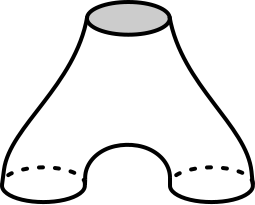
\includegraphics[scale=0.3]{../2020/pair-of-pants.png}}}
\end{equation}
\cc{In string theory,它表示上面的 strings 变成下面的 string 的「时间过程」。
}{
	which in String Theory represents the "time course" of the two strings above becoming the string below.
}

\subsection{Type theory}

\cc{描述 \emp{program} 或 \emp{computation} 的语言叫 type theory.  例如在一般的 编程语言 里可以有这样的一句:
}{
	The language that describes \emp{programs} or \emp{computation} is called type theory.  For example, the following line is typical in  common programming languages:
}
\begin{equation}
\begin{small}
\verb!define length(s: String): Integer = { .... }!
\end{small}
\end{equation}
\cc{意思是说 length() 是一个函数,输入 String,输出 Integer.
}{
	It means that length() is a function, that takes an input String, and outputs an Integer.
}

\cc{在数学里 我们描述 \emp{函数} 时会用:
}{
	In mathematics, we denote \emp{functions} by:
}
\begin{equation}
f: A \rightarrow B
\end{equation}
\cc{这个表达式其实就是 type theory 的一般形式:
}{
	This expression is actually a general form of type theory:
}
\begin{equation}
\overbrace{t}^{\mbox{term}} : \overbrace{T}^{\mbox{type}}
\end{equation}
\cc{而这个 notation $t:T$ 其实也可以写成 $t \in T$(但不正统而已)。 
}{
	And this notation $t:T$ can actually be written as $t \in T$ (though unorthodox).
}

\cc{换句话说,types 就是 \textbf{集合},terms 是集合中的 \textbf{元素}。 
}{
	In other words, a type is a \textbf{set}, and terms are the \textbf{elements} in the set.
}

\cc{更一般地,一个 type theory 的句子 可以包含 type \emp{context}:
}{
	More generally, a type theory statement can contain type \emp{contexts}:
}
\begin{equation}
\overbrace{x : A}^{\mbox{context}} \vdash \overbrace{f(x) : B}^{\mbox{type assignment}}
\end{equation}
\cc{意思就像在 program 的开头 ``declare'' 一些 变量 的类型,然后 program 就可以被 \emp{赋予} 后面的 类型。 
}{
	It is like ``declaring'' the types of variables at the beginning of a program, and then the program can be \textbf{assigned} the latter type.
}

\cc{这个 $\vdash$ 的过程 称为 \emp{type assignment},而这就是 type theory 做的全部工作。 
}{
	This $\vdash$ process is called \emp{type assignment}, and it is all that type theory does.
}

\subsubsection{$\lambda$-calculus}

\cc{在一个 program 里,除了定义 类型,还需要定义 \emp{函数}。 这件工作是由 $\lambda$-calculus 负责。
}{
	In a program, besides defining its type, you also need to define its \emp{function}.  This work is done by $\lambda$-calculus.
}

\cc{$\lambda$-calculus 可以定义函数 而不需要提及它的「名字」。 例如,用数学式表达:
}{
	$\lambda$-calculus can define functions without mentioning its ``name''. For example, in mathematical notation:
}
\begin{equation}
f(x) \triangleq x^2
\end{equation}
\cc{它的 $\lambda$-表达式就是:
}{
	Its $\lambda$-expression is:
}
\begin{equation}
f \triangleq \lambda x. \; x^2
\end{equation}
\cc{注意: 在 $\lambda$-表达式里,不需要提到 $f$ 的「名字」。
}{
	Note: In the $\lambda$-expression, there is no need to mention the ``name'' of $f$.
}

\cc{$\lambda$-calculus 是由 Alonso Church 发明,目的是研究数学上 \emp{substitution} 的性质。 Substitute 是每个中学生都懂得做的事,但要用数学表达出来却是出奇地麻烦。 
}{
	$\lambda$-calculus was invented by Alonso Church to study the properties of \emp{substitution} in mathematics.  Substitution is something every middle school student knows to do, but is surprisingly troublesome to express in mathematics.
}

\cc{同时,Church 发现 $\lambda$-calculus 是一种「万有」的计算形式,和 \emp{Turing machines} 等效。 「AI 之父」John McCarthy 用 $\lambda$-calculus 发展出 \emp{Lisp} 语言,它是所有 functional programming language 的鼻祖。 
}{
	At the same time, Church found that $\lambda$-calculus is a ``universal'' form of computation, which is equivalent to \emp{Turing machines}.  John McCarthy, the ``Father of AI'', used $\lambda$-calculus to develop the \emp{Lisp} language, which is the origin of all functional programming languages.
}

\subsubsection{Curry-Howard correspondence}

\cc{在 Curry-Howard 对应下,type $A$ 就是 逻辑命题 $A$,type $A$ 或 集合 $A$ 里面的 元素 是其 \textbf{证明} (proof, or proof witness)。
}{
	Under Curry-Howard correspondence, the type $A$ is the logic proposition $A$, and the element in type $A$ (or set $A$) is its \textbf{proof} (or proof witness).
}

\cc{而,$A \Rightarrow B$ 也是 逻辑命题,它对应於 the function type $A \rightarrow B$,也可以写作 $B^A$,而这个 type 或 集合 里面的 元素 就是一些 函数 $f: A \rightarrow B$.  如果 有一个这样的函数存在,则 type $A \rightarrow B$ 有「住客」(inhabited),换句话说 $A \Rightarrow B$ 有 \textbf{证明}。 
}{
	Also, $A \Rightarrow B$ is a logic proposition, which corresponds to the function type $A \rightarrow B$, which can also be written as $B^A$, and the elements in this type or set are certain functions $f: A \rightarrow B$.  If such functions exist, then type $A \rightarrow B$ is "inhabited", in other words $A \Rightarrow B$ has \textbf{proof}.
}

\subsection{Intuitionistic logic}

\cc{Curry-Howard isomorphism 揭示了 type theory 和 \emp{intuitionistic logic} (直觉主义逻辑)之间的关系。 这种逻辑的特点是没有 \emp{排中律} (law of excluded middle, LEM),或者等价地,\emp{double negation},即 $\neg \neg p \Rightarrow p$.
}{
	The Curry-Howard isomorphism reveals the relationship between type theory and \emp{intuitionistic logic}.  The characteristic of this logic is that there is no \emp{law of excluded middle} (LEM), or equivalently, \emp{double negation}, that is, $\neg \neg p \Rightarrow p$.
}

\cc{排中律 是说: $p \vee \neg p$ 是 恒真命题。 但在 直觉主义 逻辑中,$p \vee \neg p$ 表示 $p$ 的证明 \textbf{或} $\neg p$ 的证明,但有时候这两者都不知道(例如 现时仍未找到证明,或者不可能找到证明)。 
}{
	The law of excluded middle says $p \vee \neg p$ is a tautology.  But in intuitionistic logic, $p \vee \neg p$ means the proof of $p$ \textbf{or} the proof of $\neg p$.  Sometimes neither of them is known (for example, no proof has been found yet, or it is impossible to find such proofs).
}

\cc{附带一提: 人们惊讶地发现,在直觉主义逻辑下,axiom of choice $\Rightarrow$ law of excluded middle.  换句话说,axiom of choice 和 直觉主义 也有内在的矛盾。 
}{
	Incidentally, people are surprised to find that under intuitionistic logic, the axiom of choice $\Rightarrow$ law of excluded middle.  In other words, the axiom of choice and intuitionism have inherent contradictions.
}

\subsubsection{Topological interpretation}

\cc{在 拓樸学 里,一般用 \emp{open sets} 表示空间中的子集(这习惯起源自 Hausdorff 时期)。  但 $p$ 的 \emp{补集} $\overline{p}$ 并不 open,所以要将 $\neg p$ 定义为 $p$ 的补集的 \emp{interior},即 $\neg p \triangleq \overline{p}^{\, \circ}$.  於是 $p \cup \neg p \neq \mbox{Universe}$: \footnote{diagram from the book: \textit{Classical and Non-classical Logics -- an introduction to the mathematics of propositions} [Eric Schechter 2005], p.126.}
}{
	In topology, \emp{open sets} are generally used to represent subsets in space (this originated from the Hausdorff period).  But the \emp{complement} $\overline{p}$ of $p$ is not open, so we should define $\neg p$ as the \emp{interior} of the complement of $p$, that is, $\neg p \triangleq \overline{p}^{\, \circ}$. Thus $p \cup \neg p \neq \mbox{Universe}$: \footnote{diagram from the book: \textit{Classical and Non-classical Logics - an introduction to the mathematics of propositions} [Eric Schechter 2005], p.126.}
}
\begin{equation}
\vcenter{\hbox{\includegraphics[scale=0.8]{../2020/../2020/topology-intuitionistic.png}}}
\end{equation}

\subsection{Higher-order logic}

\cc{Propositional logic 的意思是: 只有命题,但忽略任何 \textbf{命题内部} 的结构。 
}{
	Propositional logic deals only with propositions, ignoring any \textbf{internal structure} of propositions.
}

\cc{假设 $p, q$ 是命题,命题逻辑的基本运算 就是 $p \wedge q, p \vee q, p \Rightarrow q, \neg p$.
}{
	Assuming that $p, q$ are propositions, the basic operations in propositional logic are $p \wedge q, p \vee q, p \Rightarrow q, \neg p$.
}

\cc{First-order logic 的意思是: 容许 这样的方法 构成 命题:
}{
	First-order logic allows to construct propositions like this:
}
\begin{equation}
\overbrace{\mbox{IsHuman}}^{\mbox{predicate}} ( \overbrace{\mbox{John}}^{\mbox{object}} ).
\end{equation}
\cc{Predicate 的意思是 \emp{谓词}; 谓词 是一些「有洞的命题」,它们被填入 objects 之后就变成完整的命题。 类似地可以有 \emp{多元}的 predicates,例如:
}{
	Predicates are "propositions with holes".  They become complete propositions after being filled in with objects.  Similarly, there can be predicates of \emp{multiple arity}, for example:
}
\begin{equation}
\mbox{Loves} (\mbox{John}, \mbox{Mary}).
\end{equation}
\cc{First-order 指的是: $\forall, \exists$ 这些 \emp{量词} 可以 \textbf{作用} 在 (first-class) objects 的类别上,例如(Mary \textit{人见人爱}):
}{
	The adjective ``first-order'' is related to $\forall$ and $\exists$.  These \emp{quantifiers} can \textbf{act on} all first-class objects, for example (\textit{everyone loves Mary}):
}
\begin{equation}
\forall x. \; \mbox{Loves}(x, \mbox{Mary})
\end{equation}
\cc{但 first-order logic 不容许 量词 作用在 predicates 的类别上,除非用 second-order logic.
}{
	But first-order logic does not allow quantifiers to act on predicates;  That requires second-order logic.
}

\cc{一个 二阶逻辑的例子是「\textit{拿破仑 具有一个好将军应该具备的所有特质}」:
}{
	An example of second-order logic is ``\textit{Napoleon has all the qualities that a good general should have}'':
}
\begin{equation}
\forall p. \; p(\mbox{Good General}) \Rightarrow p(\mbox{Napoleon}).
\end{equation}
\cc{注意 $p$ 是在 predicates 的类别之上量化的。
}{
	Note that $p$ is quantified over predicates.
}

\subsection{\cc{旧式 logic with type theory}{Old-style logic with type theory}}

\cc{Type theory 的历史还可以追溯更早。 它起源於 Russell 为了解决 \emp{逻辑悖论},例如:「\textit{一个只帮自己不理发的人理发的理发师帮不帮自己理发?}」  这些 逻辑悖论 根源是在於: 定义一样东西的时候,中途 \textbf{指涉} 了这个东西本身。 这种不良的定义称作 \emp{impredicative}.  为了避免不良定义,每个东西出现之前必需「宣告」它的类型,这就是 type theory 原来的目的。 
}{
	The history of Type theory can be traced back even earlier. It began with Russell's attempt to resolve \emp{logic paradoxes}, for example: ``\textit{Does a barber who only shaves people who don't shave themselves shave himself?}''  The root of these logic paradoxes stems from:  definition of something that \textbf{refers to} the thing itself.  Such a problematic definition is called \emp{impredicative}.  In order to avoid bad definitions, everything's type must be "declared" before it appears.  This is the original purpose of type theory.
}

\cc{在 Curry-Howard isomorphism 未被重视之前,有一种更简单地 用 type theory 定义 逻辑的方法。 在这种方法下,逻辑命题 $p, q, p \wedge q$ 等 \textbf{直接用} terms 定义,而不是像 Curry-Howard 那样,逻辑命题 = types,证明 = terms.
}{
	Before Curry-Howard isomorphism was taken seriously, there was a simpler way to define logic with type theory.  In this approach, the logic propositions $p, q, p \wedge q$ etc. are \textbf{defined directly} by terms, rather than via ``propositions = types, proofs = terms'' as in Curry-Howard.
}

\cc{在这情况下 type theory 处理的是 (first- or higher-order) predicate logic 的方面。 这是说,例如:
}{
	In this case, type theory deals with the aspect of (first- or higher-order) predicates.  For example, in:
}
\begin{equation}
\mbox{IsHuman} (\mbox{John})
\end{equation}
\cc{里面 IsHuman 是一个 函数 term,它输入一个 物体,输出它是不是「人」的真值 (truth value) $\in \Omega = \{ \top, \bot \}$.  因此 IsHuman 是一个 类型为 $\mbox{Obj} \rightarrow \Omega$ 的 term.
}{
	IsHuman is a function term, it inputs an object, and outputs the truth value $\in \Omega = \{ \top, \bot \}$ of whether it is a ``person''.  Therefore IsHuman is a term of type $\mbox{Obj} \rightarrow \Omega$.
}

\cc{这种做法没有容纳 Curry-Howard isomorphism 的馀地。 如果要做到后者,需要的是 Martin-L\"{o}f type theory....
}{
	This approach has no room for Curry-Howard isomorphism.  To do the latter, we would need Martin-L\"{o}f type theory....
}

\subsection{Martin-L\"{o}f type theory}
\label{sec:Martin-Lof-TT}

\cc{根据 Curry-Howard, 下面的 $A {\color{blue}\Rightarrow} B$ 是一个 逻辑命题,因而是一个 type: 
}{
	According to Curry-Howard, $A {\color{blue}\Rightarrow} B$ is a logic proposition and therefore a type:
}
\begin{equation}
\label{eqn:2-levels-of-TT}
\vcenter{\hbox{\includegraphics[scale=0.8]{../2020/why-Martin-Lof.png}}}
\end{equation}
\cc{但另方面,Human() 和 Mortal() 这两个 predicates 也需要借助 type theory 来构成命题,它们也是 types.  ${\color{red}\mbox{红色} \rightarrow}$ 和 ${\color{blue}\mbox{蓝色} \Rightarrow}$ 的两个层次 是完全不同的 两码子事,但因为 Curry-Howard 而被逼 挤在一起。 这就使得 type theory 好像「一心不能二用」。
}{
	On the other hand, Human() and Mortal() are predicates and they also need type theory to form propositions.  They are also types.  The two levels ${\color{red}\mbox{red} \rightarrow}$ and ${\color{blue}\mbox{蓝} \Rightarrow}$ are completely different, but they are forced to live together because of Curry-Howard.  It seems that type theory is ``multi-tasking''.
}

\cc{在 ``simple'' type theory 里面可以 构造:
}{
	In ``simple'' type theory one can construct:
}
\begin{itemize}
	\item sum type $A + B$

	\item product type $A \times B$

	\item function type $A \rightarrow B$
\end{itemize}
\cc{分别对应於 直觉主义逻辑的 $\vee, \wedge, {\color{blue}\Rightarrow}$.  这些是在 \textbf{命题逻辑} 层面的,已经「用尽」了 type theory 的法宝。 
}{
	They correspond to the intuitionistic logic $\vee, \wedge, {\color{blue}\Rightarrow}$.  These are at the level of \textbf{propositional logic} and they have ``exhausted the bag of tricks'' in type theory.
}

\cc{但 Human(Socrates) 也是由 Human() 和 Socrates 构成的命题,这构成的方法是用一个 arrow ${\color{red}\rightarrow}$,但已经没有 arrow 可用。 
}{
	However, Human(Socrates) is also a proposition composed of Human() and Socrates.  This requires to use an arrow ${\color{red}\rightarrow}$, but there are no more arrows available.
}

\cc{Martin-L\"{o}f 提出的解决方案是 引入新的 \emp{type constructors}:
}{
	The solution proposed by Martin-L\"{o}f is to introduce new \emp{type constructors}:
}
\begin{itemize}
	\item \textbf{dependent} sum type $\Sigma$

	\item \textbf{dependent} product type $\Pi$
\end{itemize}

\cc{Dependent sum $\displaystyle \sum_A B$ 里面 $B$ 的类型 depends on $A$. 整个 family of A 的 + 的结果变成类似 product $A \times B$.
}{
	The type of $B$ in the dependent sum $\displaystyle \sum_A B$ depends on $A$. The sum of the entire family of $A$ (indexed by $B$) is similar to the product $A \times B$.
}

\cc{Dependent product $\displaystyle \prod_A B$ 里面 $B$ 的类型 depends on $A$. 整个 family of A 的 $\times$ 的结果变成类似 exponentiation $B^A$.
}{
	The type of $B$ in the dependent product $\displaystyle \prod_A B$ depends on $A$. The product of the entire family of $A$ is similar to the exponentiation $B^A$.
}

\cc{Dependent products can be used to define \textbf{predicates} such as Human() and Mortal().  They are of type $\displaystyle \mathrm{Obj} \rightarrow \Omega = \Omega^{\mathrm{Obj}} = \prod_{\mathrm{Obj}} \Omega$.  \footnote{Note that ``objects'' here mean logic objects, not objects in category theory.}
}{
	Dependent products can be used to define \textbf{predicates} such as Human() and Mortal().  They are of type $\displaystyle \mathrm{Obj} \rightarrow \Omega = \Omega^{\mathrm{Obj}} = \prod_{\mathrm{Obj}} \Omega$.  \footnote{Note that ``objects'' here mean logic objects, not objects in category theory.}
}

\cc{一个很漂亮的结果是: 如果用 $\sum_A B$ 和 $\prod_A B$ 定义 逻辑命题,则这些 types 如果被 inhabited 的话,分别对应於 $\exists A. B(A)$ 和 $\forall A. B(A)$. 这是因为: 如果 $A \times B$ inhabited,表示\textbf{至少存在}一个 $B(A)$; 而如果 $B^A$ inhabited,则存在一个函数,将\textbf{任意的} $A$ send to $B$.
}{
	A very beautiful result is: If we use $\sum_A B$ and $\prod_A B$ to define logic propositions, these types, if inhabited, correspond to $\exists A. B(A)$ and $\forall A. B(A)$, respectively. This is because: If $A \times B$ is inhabited, it means there \textbf{exists} at least one $B(A)$; and if $B^A$ is inhabited, there is a function that sends \textbf{arbitrary} $A$'s to $B$'s.
}

Per Martin-L\"{o}f (1942-) was the first logician to see the full importance of the connection between intuitionistic logic and type theory.
\begin{equation}
\nonumber
\mbox{Per Martin-L\"{o}f (1942-)} \quad \vcenter{\hbox{\includegraphics[scale=0.5]{../2020/Martin-Lof.jpg}}}
\end{equation}

\subsection{Arithmetic-logic correspondence}

\cc{很多人都知道,经典逻辑中 $\wedge, \vee$ 对应於 \textbf{算术运算} $\times, +$(也可以看成是 fuzzy logic 的 $\min, \max$.) 其实这就是 George Boole 尝试将 \emp{逻辑} 变成 某种\emp{代数} 的原因。
}{
	Many people know that in classical logic $\wedge, \vee$ correspond to the \textbf{arithmetic operations} $\times, +$ (they also correspond to $\min, \max$  in fuzzy logic.)  Historically, that was the reason why George Boole tried to formulate \emp{logic} as some kind of \emp{algebra}.
}

\cc{较少人知道的是 $A \Rightarrow B$ 也对应於 $B^A$:
}{
	What fewer people know is that $A \Rightarrow B$ also corresponds to $B^A$:
} \footnote{I learned this from David Corfield's book \cite{Corfield}}
\begin{equation}
\label{truth-table:material-implication}
\begin{tabular}{|c|c|c|c|}
\hline 
$A$ & $B$ & $A \Rightarrow B$ & $B^A$ \\ 
\hline \hline 
0 & 0 & 1 & $0^0 = 1$ \\
\hline 
0 & 1 & 1 & $1^0 = 1$ \\ 
\hline 
1 & 0 & 0 & $0^1 = 0$ \\ 
\hline 
1 & 1 & 1 & $1^1 = 1$ \\ 
\hline 
\end{tabular} 
\end{equation}
\cc{
其中 $0^0$ 是「不确定式」,但按照 组合学 惯例可以定义为 1.
}{
where $0^0$ is ``indeterminate'', but according to combinatorics convention, it can be defined as 1.
}

\cc{这个惊奇的「巧合」似乎再一次证实 Curry-Howard correspondence 是正确的; 特别地,它意味 $\Rightarrow$ 应该看成是 \textbf{函数},即所谓 ``functional interpretation of logical deduction.'' 
}{
	This surprising "coincidence" seems to prove once again that Curry-Howard correspondence is correct;  In particular, it means that $\Rightarrow$ should be interpreted as \textbf(function), the so-called ``functional interpretation of logical deduction.''
}

\subsection{The problem of material implication}
\label{sec:material-implication}

\cc{更详细观察,table (\ref{truth-table:material-implication}) 里面 $A$ 和 $B$ 的 truth values 可以看成是它们的 types 有没有 \textbf{inhabitants}. Type $A$ 的 inhabitant 就是它的证明 $\witness$,没有证明就是 $\emptyset$.  或者推广到:命题 $A$ 的真值 = $A$ 的 type 作为 集合 的 \textbf{cardinality}; The truth valuation of $A = |A|$.  这样看,$A \Rightarrow B$ 的真值 就是 $|B^A|$, 亦即是从 $\{\witness\}$ 或 $\emptyset$ 到 $\{\witness\}$ 或 $\emptyset$ 的 map 的\textbf{个数}, 而这个 map 只有在 $ \{\witness\} \mapsto \emptyset$ 的时候是空集(不可能)。
}{
	To observe in more detail, the truth values of $A$ and $B$ in table (\ref{truth-table:material-implication}) can be regarded as whether their types have \textbf{inhabitants}.  A type's inhabitant is its proof $\witness$, whereas $\emptyset$ means no proof.  More abstractly:  the truth value of the proposition $A$ = the \textbf{cardinality} of the type $A$ as a set; $|A|$.  In this way, the true value of $A \Rightarrow B$ is $|B^A|$, that is, the \textbf{number} of maps from $\{\witness\}$ or $\emptyset$ to $\{\witness\}$ or $\emptyset$, and such maps is the empty set only in the case $\{\witness\} \mapsto \emptyset$ (which is impossible).
}

\cc{这个观察 可以推广到 fuzzy logic (\S\ref{sec:fuzzy-implication}) 和 strict implication $A \strictif B$ (\S\ref{sec:strict-implication}).
}{
	This observation may be extended to fuzzy logic (\S\ref{sec:fuzzy-implication}) and strict implication $A \strictif B$ (\S\ref{sec:strict-implication}).
}

\cc{但 material implication 导致某种悖论:
}{
	However, material implication seems to lead to a certain fallacy:
}
\begin{equation}
A \wedge B \quad \vdash \quad A \Rightarrow B
\end{equation}
\cc{例如
}{
For example,
}
\begin{equation}
\mbox{\cc{看见黑猫}{seeing black cat}} \wedge \mbox{\cc{发生车祸}{car accident}} \quad \vdash \quad \mbox{\cc{看见黑猫}{seeing black cat}} \Rightarrow \mbox{\cc{发生车祸}{car accident}}
\end{equation}
\cc{即任何两件\textbf{同时}发生的事件,会导致类似\textbf{因果}的结论,然而这因果关系未必成立。 这个谬误出现的原因,似乎是因为混淆了不同时间的 \emp{cases}.  换句话说: 我们应该验证了 table (\ref{truth-table:material-implication}) 的所有 cases,然后才下结论说 $A \Rightarrow B$; 然而根据 经典逻辑的 material implication,只需要一个 case 就可以下结论说 $A \Rightarrow B$.
}{
	That is to say, any two \textbf{coincidental} occurrences will lead to a conclusion similar to \textbf{causality}, even though this causal relationship may not exist.  This fallacy seems stem from the confusion of \textbf{cases at different times}.  In other words:  We should verify all the cases in table (\ref{truth-table:material-implication}) before drawing the conclusion $A \Rightarrow B$;  However, according to classical logic, only one case is needed to establish that $A \Rightarrow B$.
}

\cc{那么,这个谬误 为什么没有在 经典逻辑 AI 系统中被发现?
}{
	So, why is this flaw not discovered in classic logic AI systems?
}

\cc{所谓 \textbf{inductive learning of logic rules},其原理是根据以下的「生成模型」: 
}{
	The principle of the so-called \textbf{inductive learning of logic rules} is based on the following ``generative model'':
}
\begin{equation}
\begin{tikzcd}[| /.tip = {Bar[scale=3]}, column sep = large]
\mbox{generators} \arrow[|-,r, "\mathrm{generate}"]
& \mbox{data of the world}
\end{tikzcd}
\end{equation}
\cc{这种 generators 的思想,和 数学中 generators of ideals, groups, function fields, 等 是一样的。 
}{
	The idea behind such ``generators'' is the same as generators of ideals, groups, function fields, etc. in mathematics.
}

\cc{Machine learning 的目的,是求得一组这样的 generators,而它生成的\textbf{机制},即是逻辑推导 $\vdash$.
}{
	The purpose of machine learning is to obtain a set of such generators, and the \textbf{generating mechanism} is logic derivation, $\vdash$.
}

\cc{但由於在 learning 的过程中,需要验证 \textbf{不同时间}的 cases,因此避免了 太轻易接受 $A \Rightarrow B$ 的问题。 
}{
	However, since the cases (occurring at \textbf{different times}) need to be verified during the learning process, the problem of accepting $A \Rightarrow B$ too easily is avoided.
}

\section{Topos theory}

\subsection{Basics}

\cc{将 type theory 对应到 category theory,这工作是 Lambek 做的,於是完成了 Curry-Howard-Lambek 的「三位一体」:
}{
	Making a connection between type theory and category theory, this work was done by Lambek, thus creating a Curry-Howard-Lambek ``Trinity'':
}
% \tikzcdset{arrows={line width=3pt}}
\begin{equation}
\begin{tikzcd}[column sep = -1em]
\mbox{logic} \arrow[-,rr,line width=1.5pt] \arrow[-,dr]
&& \mbox{programming} \arrow[-,dl] \\
& \mbox{category theory}
\end{tikzcd}
\end{equation}

\begin{equation}
\nonumber
\mbox{Joachim Lambek (1922-2014)} \quad \vcenter{\hbox{\includegraphics[scale=0.4]{../2020/Lambek.jpg}}}
\end{equation}

\cc{Topos 的重要意义在於 它是一个可以用来 \textbf{进行逻辑运算} 的范畴,关键在於它可以表达 \textbf{子集} 的概念,或更一般地叫作 \emp{sub-objects}.
}{
	The significance of topos is that it is a category in which one can perform \textbf{logic / set-theoretic operations}.  The key is that it can express the concept of \textbf{sub-sets}, or more generally called \emp{sub-objects}.
}

\cc{一个 topos $\mathcal{C}$ 里面存在 sub-object classifer $\Omega$ 使得 $X \rightarrow \Omega \cong \mbox{sub-objects of } X$.  换句话说 $X$ 的 子集 可以用 $X \rightarrow \Omega$ 这个映射来 \emp{represent}.
}{
	Every topos $\mathcal(C)$ has a sub-object classifer $\Omega$, so that $X \rightarrow \Omega \cong \mbox{sub-objects of} X$.  In other words, a subset of $X$ can be represented by the map $X \rightarrow \Omega$.
}

\cc{在 $\mathbf{Set}$ 这个 topos 里面,$\Omega$ 是一个有\textbf{两个}元素的集合,可以记作 $\{ \top, \bot \}$.  那么 $X \rightarrow \Omega$ 就是一些 \emp{命题},例如 $X$ 是人的集合,则 $\begin{tikzcd}[ampersand replacement=\&, column sep = 12ex] X \arrow[r, "\mathrm{mathematician}"] \& \Omega \end{tikzcd}$ 定义哪些人是数学家。 
}{
	In the topos of $\mathbf{Set}$, $\Omega$ is a set of \textbf{two} elements, which can be written as $\{ \top, \bot \}$.  Maps like $X \rightarrow \Omega$ are \emp{propositions}.  For example, if $X$ is a collection of people, then $\begin{tikzcd}[ampersand replacement=\&, column sep = 12ex]
	X \arrow[r, "\mathrm{mathematician}"] \& \Omega \end{tikzcd}$ defines who is a mathematician.
}

\cc{Topos theory 里面最重要的 commutative diagram 是这个:
}{
	The most important commutative diagram in Topos theory is this:
}
\begin{equation}
\label{eqn:subobject-classifier}
\begin{tikzcd}[column sep = normal]
X \arrow[r, "!"] \arrow[d, tail, swap, "m"] & 1 \arrow[d, "\mathrm{true}"] \\
Y \arrow[r, swap, "\Chi_m"] & \Omega
\end{tikzcd}
\end{equation}
\cc{其中:
}{
	where:
}
\begin{itemize}
	\cc{\item $X \stackrel{!}{\longrightarrow} 1$ 是个 unique arrow,它将 集合 $X$ \textbf{整个地}映射到 1. 而 1 是 terminal object,它的定义就是说,通向它的箭咀只能有一个。
	}{
		\item $X \stackrel{!}{\longrightarrow} 1$ is a unique arrow, which maps the set $X$ \textbf{entirely} to 1.  1 is the \emp{terminal object}, which is defined by saying there can only be one arrow leading to it.
	}
	
	\cc{\item $\begin{tikzcd}[ampersand replacement=\&] 1 \arrow[r, "\mathrm{true}"] \& \Omega \end{tikzcd}$ 在 $\top$ 和 $\bot$ 之间选择 $\top$, 因此叫 ``true'' arrow.
	}{
		\item $\begin{tikzcd}[ampersand replacement=\&] 1 \arrow[r, "\mathrm{true}"] \& \Omega \end{tikzcd}$ picks out $\top$ between $\top$ and $\bot$, so we call it the ``true'' arrow.
	}
	
	\cc{\item $\begin{tikzcd}[ampersand replacement=\&] X \arrow[r, tail, "m"] \& Y \end{tikzcd}$ 是 \emp{monic} arrow,特别地,在 $\mathbf{Set}$ 里面它就是 \emp{inclusion} map,即 $\begin{tikzcd}[ampersand replacement=\&] X \arrow[r, hook, "m"] \& Y \end{tikzcd}$.  它表示 $X$ 是 $Y$ 的\textbf{子集},$X \subseteq Y$.
	}{
		\item $\begin{tikzcd}[ampersand replacement=\&] X \arrow[r, tail, "m"] \& Y \end{tikzcd}$ is a \emp{monic} arrow;  Particularly, in $\mathbf{Set}$ it is the \emp{inclusion map}, ie $\begin{tikzcd}[ampersand replacement=\&] X \arrow[r, hook, "m"] \& Y \end{tikzcd}$.  It means that $X$ is a \textbf{subset} of $Y$, $X \subseteq Y$.
	}

	\cc{\item $\begin{tikzcd}[ampersand replacement=\&] Y \arrow[r, "\Chi_m"] \& \Omega \end{tikzcd}$ 是集合论中熟悉的 \emp{characteristic function}, 当元素 $e \in X \subseteq Y$ 时,$\Chi(e)$ 取值 1,否则为 0.  正是 $\Chi_m$ 的存在令这幅图 commute.  $\Chi_m$ 也记作 $\ulcorner m \urcorner$.
	}{
		\item $\begin{tikzcd}[ampersand replacement=\&] Y \arrow[r, "\Chi_m"] \& \Omega \end{tikzcd}$ is the familiar \emp{characteristic function} in set theory.  When the element $e \in X \subseteq Y$, $\Chi(e)$ takes the value 1, otherwise it is 0.  It is the existence of $\Chi_m$ that makes this diagram commute.  $\Chi_m$ is also denoted $\ulcorner m \urcorner$.
	}
\end{itemize}
\cc{不熟悉基本范畴论的读者,我非常推荐看一看《Conceptual Mathematics》这本书,写得连中学生也可以看懂,而作者之一的 Lawvere 正是 topos 理论的创始人。 
}{
	For readers who are not familiar with basic category theory, I highly recommend the book \textit{Conceptual Mathematics}, written in a style even high school students can understand.  One of the authors is Lawvere, creator of topos theory.
}

\cc{从 $\mathbf{Set}$ 的角度看,这个 diagram 很易理解,但 topos 的好处是它可以将这些逻辑概念 \textbf{generalize} 到比 $\mathbf{Set}$ 更一般的范畴。 
}{
	From the perspective of $\mathbf{Set}$, this diagram is easy to understand, but the advantage of topos is that it can \textbf{generalize} these logical concepts to a more general category than $\mathbf{Set}$.
}

\cc{Topos 理论的重要性 在於 它用 category 的语言 \textbf{重新表述}了 集合论的整个基础。 特别地,逻辑学中的符号,例如 $P(x), \forall x, \exists x,$ 表面上看似无法用范畴论表示,这正是 Lawvere 惊人的成就。 
}{
	The importance of the Topos theory is that it uses the language of category to \textbf{re-formulate} the entire basis of set theory.  In particular, the symbols in logic, such as $P(x), \forall x, \exists x$, seemed impossible to express in category theory.  This is Lawvere's amazing achievement.
}
\begin{equation}
\nonumber
\mbox{William Lawvere (1937-)} \quad 
\vcenter{\hbox{\includegraphics[scale=1.0]{../2020/Lawvere.jpg}}}
\end{equation}

\cc{再看一次 图 (\ref{eqn:subobject-classifier}):
}{
	Look again at the commutative diagram (\ref(eqn:subobject-classifier)):
}
\begin{equation}
\begin{tikzcd}[column sep = normal]
X \arrow[r, "!"] \arrow[d, tail, swap, "m"] \arrow[dr, phantom, "\lrcorner", red, very near start] & {\color{red}1} \arrow[d, red, "\mathrm{true}"] \\
Y \arrow[r, swap, "\ulcorner m \urcorner"] & {\color{red}\Omega}
\end{tikzcd}
\end{equation}
\cc{右边的 ${\color{red}\mathrel{\substack{1\\\downarrow\\\Omega}}}$ 称为 \emp{generic subobject}.  它的 \emp{pull back} square 用 ${\color{red}\lrcorner}$ 记号表示。 而左边的 $\mathrel{\substack{X\\\downarrow\\Y}}$ 则是一般的 sub-object. We say that the \textbf{property} of being a sub-object is \emp{stable under pullbacks}.
}{
	The ${\color{red}\mathrel{\substack{1\\\downarrow\\\Omega}}}$ on the right is called the \emp{generic subobject}.  Its \emp{pull back} square is indicated by ${\color{red}\lrcorner}$.  And the $\mathrel{\substack{X\\\downarrow\\Y}}$ on the left is a general sub-object.  We say that the \textbf{property} of being a sub-object is \emp{stable under pullbacks}.
}

\subsection{$\forall$ and $\exists$ as adjunctions}

Let $\mbox{Forms}(\bar{X})$ denote the set of formulas with only the variables $\bar{X}$ free. ($\bar{X}$ may contain multiple variables.)

Then one can always trivially add an additional \textbf{dummy} variable $Y$:
\begin{equation}
\delta : \mbox{Forms}(\bar{X}) \rightarrow \mbox{Forms}(\bar{X}, Y)
\end{equation}
taking each formula $\Phi(\bar{X})$ to itself.

It turns out that $\exists$ and $\forall$ are \textbf{adjoints} to the map $\delta$:
\begin{equation}
\begin{tikzcd}[column sep = large]
\mbox{Forms}(\bar{X}) 
\arrow[r, "\delta"]
& \mbox{Forms}(\bar{X},Y) 
\arrow[l, shift right=1.2em, "\exists_Y"'] % "\bot"
\arrow[l, shift left=1em, "\forall_Y"] % "\bot"'
\end{tikzcd}
\end{equation}
\cc{or simply denoted as $\exists \dashv \delta \dashv \forall$.  而这是十分 makes sense 的,因为 一个 $\Phi(\bar{X},Y)$ 的式子,经过 $\forall Y. \; \Phi(\bar{X},Y)$ 之后,就变成一个和 $Y$ \textbf{无关}的式子。
}{
	or simply denoted as $\exists \dashv \delta \dashv \forall$.  And this makes a lot of sense, because a formula $\Phi(\bar{X},Y)$, after being quantified by $\forall Y. \; \Phi(\bar{X},Y)$, becomes a formula that is \textbf{independent} of $Y$.
}

\cc{In \textbf{cylindric algebra}, the quantifiers $\forall_Y$ and $\exists_Y$ can be interpreted as \textbf{projections} where $Y$ is the component that is ``killed'' by the projections:
}{
	In \textbf{cylindric algebra}, the quantifiers $\forall_Y$ and $\exists_Y$ can be interpreted as \textbf{projections} where $Y$ is the component that is ``killed'' by the projections:
}
\begin{equation}
\vcenter{\hbox{\includegraphics[scale=0.7]{../2020/cylindrification-projected.png}}}
\end{equation}

\cc{另一个方法是 借助 $T$ 定义
}{
	Another way is to define with the help of a variable set $T$
}
\footnote{This formula is from \parencite{Abramsky2011} }
\cc{(注意 在下图中 $\bar{X}$ 和 $Y$ 变成平面):
}{
	(Note that $\bar{X}$ and $Y$ are show as 2D domains below) :
}
% \color[rgb]{0.0,0.5,0.0}  %% dark blue
\begin{eqnarray}
\label{eqn:Abramsky-1}
\forall T \subseteq \bar{X}: \qquad 
&S \subseteq \delta^{-1} (T) \qquad \Longleftrightarrow \qquad \exists {}_Y  S \subseteq T& \\
&\vcenter{\hbox{\includegraphics[scale=0.7]{../2020/Lawvere-quantifier-exists.png}}}& \nonumber
\end{eqnarray}
\cc{熟悉 Galois theory 的读者 可以理解 adjunction 是 \textbf{Galois connection} 的推广形式。 用日常语言讲: 我们知道 $S$,想定义 $\exists S$; $S$ 存在於论域 $Y$,$\exists S$ 存在於 论域 $\bar{X}$; 借助「影子」$T$ 在 论域 $\bar{X}$ 夹著 $\exists S$,则影子的「原象」在论域 $Y$ 夹著 $S$.  下图是 $\delta$ 是 projection 的特例, $\delta$ 是「杀掉」$Y$ 的 projection:
}{
	Readers familiar with Galois theory may understand adjunctions as a generalization of \textbf{Galois connections}.  In everyday language:  We know $S$, and would like to define $\exists S$.  $S$ lives in the domain  $Y$, $\exists S$ in the domain $\bar{X}$.  We seek the help of a ``shadow'' $T$ in domain $\bar{X}$ to get ahold of $\exists S$, and the shadow's ``original'' in domain $Y$ would be holding $S$.  The following is a special case where $\delta$ is a projection, one that ``kills'' the dimension $Y$:
}
\begin{equation}
\label{fig:Lawvere-cylindrification-exists}
\vcenter{\hbox{\includegraphics[scale=0.7]{../2020/Lawvere-cylindrification-exists.png}}}
\end{equation}
\cc{注意: (\ref{fig:Lawvere-cylindrification-exists}) 的 $\delta$ 是 $\bar{X} \times Y \rightarrow X$ 的 projection,但 (\ref{eqn:Abramsky-1}) 的 $\delta$ 可以是\textbf{任何} $Y \rightarrow X$ 的映射,这似乎是 $\forall$ 和 $\exists$ 的最一般的定义。 范畴论 定义 的好处是 方便推广到其他逻辑「模型」,例如 过渡到 Banach space.
}{
	Note that in (\ref{fig:Lawvere-cylindrification-exists}), $\delta$ is a projection from $\bar{X} \times Y \rightarrow X$, but the $\delta$ in (\ref{eqn:Abramsky-1}) can be \textbf{any} map $Y \rightarrow X$, and this seems to be the most general definition of $\forall$ and $\exists$.  The advantage of using categorical definitions is that they can be easily transferred to other categories, such as Hilbert space.
}

\cc{类似地有 $\forall$ 的定义:
}{
	Similarly we have the definition of $\forall$:
}
\begin{eqnarray}
\forall T \subseteq \bar{X}: \qquad 
&\delta^{-1} (T) \subseteq S \qquad \Longleftrightarrow \qquad T \subseteq \forall {}_Y S& \\
&\vcenter{\hbox{\includegraphics[scale=0.7]{../2020/Lawvere-quantifier-forall.png}}}& \nonumber
\end{eqnarray}
\begin{equation}
\vcenter{\hbox{\includegraphics[scale=0.7]{../2020/Lawvere-cylindrification-forall.png}}}
\end{equation}

\subsection{$\wedge$ and $\Rightarrow$ as product-hom adjunction}

\cc{一个只有原子命题的逻辑系统是「静止」的,不能推出新的结论: 
}{
	A logical system with only atomic propositions is ``stationary'' and cannot draw new conclusions:
}
\begin{eqnarray}
A & \qquad & A \nonumber \\
B & \quad \vdash \quad & B \\
C & \qquad & C \nonumber
\end{eqnarray}
\cc{但如果左边加多一个式子 $A \Rightarrow D$,则可以推出新的结论 $D$:
}{
	But if a conditional formula $A \Rightarrow D$ is added to the left, a new conclusion $D$ can be drawn:
}
\begin{eqnarray}
\label{eqn:deduction}
A & \qquad & A \nonumber \\
B & \quad \vdash \quad & B \\
C & \qquad & C \nonumber \\
& \hspace*{-3em} {\color{red}A \Rightarrow D} \qquad & D \nonumber
\end{eqnarray}
\cc{换句话说,$\Rightarrow$ 算符 是逻辑引擎的「燃料」,没有它不能推动逻辑 inference 的过程。 
}{
	In other words, the $\Rightarrow$ operator is the "fuel" of a logic engine, without which the process of logic inference cannot ``run''.
}

\cc{$\vdash$ 的功能和 $\Rightarrow$ 类似,但 $\vdash$ 是 \textbf{元逻辑} (meta-logic) 的符号,而 $\Rightarrow$ 是逻辑\textbf{之内}的算符。
}{
	The function of $\vdash$ is similar to $\Rightarrow$, but $\vdash$ is a \textbf{meta-logic} symbol, whereas $\Rightarrow$ is an operator within logic.
}

\cc{在 (\ref{eqn:deduction}) 中,${\color{red} A \Rightarrow D}$ 导致了 $A \vdash D$ 的出现。
}{
	In (\ref{eqn:deduction}), ${\color{red} A \Rightarrow D}$ led to the appearance of $A \vdash D$.
}

\cc{一般来说,$\Delta \Rightarrow \Gamma$ 就是 $\vdash$ 这个映射 对於 $\Delta$ 的一个 \emp{截面} (a restriction of the $\vdash$ map to the domain $\Delta$).  这一点很重要: 一个 map 作用在某些元素上,但这些元素 和那个 map 是「同类」的。 这其实是逻辑结构的一个 defining characteristic.
}{
	Generally speaking, $\Delta \Rightarrow \Gamma$ is a \emp{section} of the mapping $\vdash$ by $\Delta$ (a restriction of the $\vdash$ map to the domain $\Delta$).  This is very important:  a map acts on certain elements, but the elements and the maps are ``on the same footing''.  This is actually a defining characteristic of logic structure.
}

\cc{在 topos 里有一个很重要的 \emp{product-hom adjunction},  它说的是 $A \wedge B$ 和 $A \Rightarrow B$ 之间的邻接:
}{
	There is a very important \emp{product-hom adjunction} in topos, which refers to the adjacency between $A \wedge B$ and $A \Rightarrow B$:
}
\begin{equation}
(A \times B) \rightarrow C \quad \simeq \quad A \rightarrow (B \rightarrow C)
\end{equation}
\cc{这在逻辑上 是见惯的,没有什么稀奇,它推论 $A \Rightarrow B$ 可以替代 $A \vdash B$.  由於 $\vdash$ 在我们的 AI 系统中是 \textbf{神经网络},这表示 神经网络中的「黑箱」知识可以「外在化」(externalize) 成 \textbf{逻辑命题},这一点 在智能系统中 是有关键的重要性,因为它表示 知识可以透过语言学习得到(虽然这也不是必需 范畴论 才可以看得出来。) 
}{
	This is nothing unusual in logic.  It means that $A \Rightarrow B$ can replace $A \vdash B$.  Since $\vdash$ is a \textbf{neural network} in our AI system, this means the ``black box'' knowledge in the neural network can be ``externalized'' as \textbf{logic propositions}, which is of key importance in intelligent systems, because it means that knowledge can be obtained through \textit{learning via language} (Although one does not necessarily need category theory to see it.)
}

\subsection{Classifying topos $\leftrightharpoons$ internal language}

\cc{想认识一个\textbf{范畴},最重要的是问: 它的 objects 是啥? 它的 morphisms 是啥? 
}{
	To understand a \textbf{category}, the most important questions are:  What are its objects? What are its morphisms?
}

\cc{Lambek 给出的对应是:
}{
	The correspondence given by Lambek is:
}
\begin{itemize}
	\item types $\leftrightsquigarrow$ objects
	\item terms $\leftrightsquigarrow$ morphisms
\end{itemize}

We have the following transformations between two formalisms:
\begin{equation}
\begin{tikzcd}[column sep = 20ex]
\boxed{\mbox{topos}} \; \mathcal{C}
\arrow[r, shift left, "\mbox{internal language}"]
& T \; \boxed{\mbox{type theory}}
\arrow[l, shift left, "\mbox{classifying topos}"]
\end{tikzcd}.
\end{equation}
In other words,
\begin{equation}
\mathcal{C} = \mathcal{C}\ell(T), \quad T = \mathrm{Th}(\mathcal{C}).
\end{equation}

\subsection{Yoneda lemma}

\begin{equation}
\nonumber
\mbox{\cc{米田 信夫}{Nobuo Yoneda} (1930-1996)} \quad 
\vcenter{\hbox{\includegraphics[scale=0.2]{../2020/Yoneda.jpg}}}
\end{equation}

\cc{在一个范畴 $\mathcal{C}$ 里面,考虑 其中一个物体 $A$ 到其他物体的 morphism, $A \rightarrow \bullet$.  这可以说是,透过 $A$「看」其他物体的方法。
}{
	In a category $\mathcal{C}$, consider the morphisms from one object $A$ to other objects, $A \rightarrow \bullet$.  This is like ``seeing'' other objects through $A$.
}

\cc{\textbf{例:} 在 $\mathbf{Set}$ 里面,$1 \rightarrow X$ 是用 终点物体 1「看」其他物体,看到的是集合的 \textbf{元素}。
}{
	\textbf{Example:} In $\mathbf{Set}$, $1 \rightarrow X$ means to ``look at'' other objects through 1, and what you see is the set of \textbf{elements}.
}

\cc{\textbf{例:} 映射 $\mathbb{R} \rightarrow X$ 是 空间 $X$ 中的 \textbf{曲线},可以说 $\mathbb{R}$「看到」曲线。
}{
	\textbf{Example:} A mapping $\mathbb{R} \rightarrow X$ is a \textbf{curve} in the space $X$.  It can be said that $\mathbb{R}$ ``sees'' curves.
}

\cc{\textbf{例:} 在 ordered set $(\mathbb{R}, \le)$ 里面 物体 $0 \rightarrow x$ 可以「看到」$x$ 是不是 \textbf{positive}.
}{
	\textbf{Example:}  In the ordered set $(\mathbb{R}, \le)$ the object $0 \rightarrow x$ can ``see'' whether $x$ is \textbf{positive}.
}

\cc{类似地,可以考虑 对偶 的情况,$\bullet \rightarrow A$ 是其他物体怎样「看」$A$ 的方法。
}{
	Similarly, we can consider the dual case, $\bullet \rightarrow A$ is how other objects ``see'' $A$.
}

\cc{\textbf{例:} 在 $\mathbf{Set}$ 里面,$X \rightarrow 2$ 是其他物体「看」2 的方式,得到的是 $X$ 的\textbf{子集}, $\powerset(X)$. 
}{
	\textbf{Example:}  In $\mathbf{Set}$, $X \rightarrow 2$ is the way other objects ``see'' 2 and what you get is the \textbf{subsets} of $X$, $\powerset(X)$.
}

\cc{\textbf{例:} 在 $\mathbf{Top}$ 里面,2 包含一个 open set 和一个 closed set,$X \rightarrow 2$ 得出的是 $X$ 的\textbf{开子集},$\mathrm{Opens}(X)$.
}{
	\textbf{Example:}  In $\mathbf{Top}$, 2 contains an open set and a closed set, $X \rightarrow 2$ sees the \textbf{open subsets} of $X$, $\mathrm{Opens}(X)$.
}

A functor $X: \mathcal{A} \rightarrow \mathbf{Set}$ is \emp{representable} if $X \cong H^A$ for some $A \in \mathcal{A}$.

\cc{$H^A$ 的意思是 $\mathcal{A}(A, -)$, 这是一个集合。 
}{
	$H^A$ denotes $\mathcal{A}(A, -)$;  This is a set.
}

A \emp{representation} of $X$ is a choice of an object $A \in \mathcal{A}$ and an isomorphism between $H^A$ and $X$.

\underconst

\emp{Yoneda embedding} of $\mathcal{A}$:
\begin{equation}
H_{\bullet}: \mathcal{A} \rightarrow [\mathcal{A}^{\mathrm{op}} , \mathbf{Set}]
\end{equation}

\begin{align}
\mbox{For each } A \in \mathcal{A} \mbox{, we have a functor} \quad
& \mathcal{A} \stackrel{H^A}{\longrightarrow} \mathbf{Set} \nonumber \\
\mbox{Putting them all together gives a functor} \quad
& \mathcal{A}^{\mathrm{op}} \stackrel{H^{\bullet}}{\longrightarrow} [\mathcal{A} , \mathbf{Set}] \\[10pt]
\mbox{For each } A \in \mathcal{A} \mbox{, we have a functor} \quad
& \mathcal{A}^{\mathrm{op}} \stackrel{H_A}{\longrightarrow} \mathbf{Set} \nonumber \\
\mbox{Putting them all together gives a functor} \quad
& \mathcal{A} \stackrel{H_{\bullet}}{\longrightarrow} [\mathcal{A}^{\mathrm{op}} , \mathbf{Set}] \nonumber
\end{align}

\begin{equation}
\begin{tikzcd}
\mathcal{A}^{\mathrm{op}} 
\arrow[r, bend left=30, "H_A"]
\arrow[r, bend right=30, swap, "X"]
\arrow[r, phantom, "\Downarrow"]
& \mathbf{Set}
\end{tikzcd}
\end{equation}

\emp{Yoneda lemma}:
\begin{equation}
[\mathcal{A}^{\mathrm{op}} , \mathbf{Set}] (H_A, X) \cong X(A)
\end{equation}

\{ How sheaves give rise to representables.... \}

\subsubsection{Application: continuation-passing style}

There is an isomorphism between the types $a$ and $\forall r. (a \rightarrow r) \rightarrow r$.  It follows from the Yoneda lamma.

In the theory of functional programming, the type $\forall r. (a \rightarrow r) \rightarrow r$ is also known as the \textbf{continuation-passing style} (CPS) of the type $a$.

Intuitively, CPS can be understood as saying that having a value is just as good as having a function that will give that value to a callback.

CPS is of special interest to logic, because it allows to extend the Curry-Howard correspondence from intuitionistic logic to \textbf{classical} logic.

\{ Explain CPS in functional programming... \}

There exists a \textbf{Kolmogorov translation} $k(\cdot)$ that converts a proposition such that (basically) each atom is preceded by a double negation ($\neg \neg$).  This translation has the property that
\begin{equation}
\phi \mbox{ provable in classical logic} \Leftrightarrow k(\phi) \mbox{ provable in intuitionistic logic.}
\end{equation}
The Kolmogorov translation is a special case of CPS.

\subsubsection{(Application?) symmetric neural networks}

\cc{(我觉得这个可能是 Yoneda lemma 的一个应用,但根据 MathOverflow 上一些专家的看法,只是表面上有点相似。
}{
	(I thought this could be an application of Yoneda lemma, but according to some experts on MathOverflow, the resemblance is only superficial.)
}

The \textbf{Kolmogorov–Arnold representation theorem} states that every multivariate continuous function can be represented as a sum of continuous functions of one variable:
\begin{equation}
f(x_1,... ,x_n) = \sum_{q=0}^{2n}\Phi_{q} \left(\sum_{p=1}^n \phi_{q,p}(x_p) \right)
\end{equation}
It can be specialized to such that every symmetric multivariate function can be represented as a sum of (the same) functions of one variable:
\begin{equation}
\label{symmetric-functions}
f(x_1, ..., x_n) = g(h(x_1) + ... + h(x_n))
\end{equation}

Cayley's theorem:  Any group can be represented as a sub-group of a special group, namely the permutation group.

Any symmetric function can be represented as a sub-function of a special symmetric function, namely the sum.

\subsection{Model theory, functorial semantics}

Model theory is basically a \textbf{functorial} map from logic formulas to algebraic objects:

\begin{equation}
\tikzmark{a1} a \tikzmark{c1} \; {\color{red}\cdot} \; \tikzmark{b1} b \longmapsto \llbracket \tikzmark{a2} a \rrbracket \tikzmark{c2} \; {\color{red}\cdot} \; \llbracket \tikzmark{b2} b \rrbracket
\begin{tikzpicture}[overlay, remember picture, distance=1.1cm]
\draw[->, out=45, in=135, transform canvas={shift={(4pt,15pt)}}] (a1.center) to (a2.center);
\draw[->, out=45, in=135, transform canvas={shift={(4pt,15pt)}}] (b1.center) to (b2.center);
\draw[->, out=-45, in=-135, transform canvas={shift={(6pt,-2pt)}}, red] (c1.center) to (c2.center);
\end{tikzpicture}
\end{equation}

On the left side is a syntactic formula (eg. logic formula), and on the right side is an object composed of elements in an algebraic \textbf{language} or \textbf{structure}.

For example, if we want to define an \textbf{Abelian group}, we would have a (syntactic) axiom that says:
\begin{equation}
a \cdot b = b \cdot a
\end{equation}
which expresses a formal (syntactic) rule concerning its symbols.  Using model theory, the syntactic object such as $a \cdot b$ is mapped to the actual algebraic objects, ie, the elements of an Abelian group.  Crucially, the multiplication symbol $\cdot$ is also mapped to the group multiplication operation.  We say that such a mapping is \textbf{functorial} --- it maps elements to elements and operations to operations.

This is the main idea behind functorial semantics.

We interpret formulas in a topos $\mathcal{E}$ by assigning each an \emp{extension}.  In topos theory this is called \emp{internal} semantics.  Note the terminology is a bit confusing.

\subsection{Generalized elements}

\cc{一个 逻辑命题 $\phi$ 可以看成是由 某论域 $A \stackrel{\phi}{\rightarrow} \Omega$ 的函数,其中 $\Omega = \{ \top, \bot \}$.
}{
	A logic proposition $\phi$ can be regarded as a function from a certain domain $A \stackrel{\phi}{\rightarrow} \Omega$, where $\Omega = \{ \top, \bot \}$.
}

\cc{也可以说:命题 $\phi(x)$ 是真的,其中 $x$ 是 $A$ 的\emp{元素}。
}{
	Another way to put it is that the proposition $\phi(x)$ is true, where $x$ is an \emp{element} of $A$.
}
In category theory, we use the terminal object $1$ to ``pick out'' elements of $A$, as follows:
\begin{equation}
1 \stackrel{x}{\rightarrow} A \stackrel{\phi}{\rightarrow} \Omega.
\end{equation}
\cc{In $\mathbf{Set}$, 任意一个由 1 出发的函数 $x: 1 \rightarrow A$ 可以直接看成是 $A$ 的「元素」。
}{
	In $\mathbf{Set}$, any map from 1, $x: 1 \rightarrow A$, can be directly regarded as an ``element'' of $A$.
}

\cc{但如果我们用另一个 论域 $C$ 取代 1,换句话说:
}{
	But if we replace 1 with another domain $C$, as in:
}
\begin{equation}
C \stackrel{x}{\rightarrow} A \stackrel{\phi}{\rightarrow} \Omega.
\end{equation}
\cc{这样的 $x: C \rightarrow A$ 叫作 $A$ 的 \emp{generalized element}.
}{
	Such an $x: C \rightarrow A$ is called a \emp{generalized element} of $A$.
}

\cc{另一个术语是: $C$ \emp{forces} $\phi(x)$, notation: $C \Vdash \phi(x)$.  这术语来自 Paul Cohen 为了解决 Continuum Hypothesis 而提出的 forcing 技巧,见 \S\ref{sec:forcing}.
}{
	Another terminology is to say that $C$ \emp{forces} $\phi(x)$, notation: $C \Vdash \phi(x)$. This comes from the forcing technique, first invented by Paul Cohen, to solve the Continuum Hypothesis, see \S\ref{sec:forcing}.
}

\cc{另一个说法是: $\phi(x)$ is true \emp{at stage} $C$. (这术语来自 possible-world semantics)
}{
	Yet another way to put it is that $\phi(x)$ is true \emp{at stage} $C$. (This comes from possible-world semantics.)
}

\subsection{Internal vs external semantics}

\cc{假设 $\phi(\bullet)$ 是一个谓词,$\phi$ 的论域 (domain) 是 $A$.  例如 $\phi(x)$ 表示 $x$ 是男性,$x \in$ 人。  则 $\phi(x)$ 这个命题的 \emp{extension}(外延)就是在「人」的集合中属於「男性」的元素。 
}{
	Suppose $\phi(\bullet)$ is a predicate, and the domain of $\phi$ is $A$. For example, $\phi(x)$ means $x$ is male and $x \in$ people.  Then the \emp{extension} of the proposition $\phi(x)$ are the elements that are ``male'' in the set ``people''.
}

\cc{知道了 $\phi$ 的 extension 就可以判断,对每一个 $x \in A, \phi(x)$ 的真假。  换句话说,提供了一种 \emp{interpretation} 的方法。 
}{
	Knowing the extension of $\phi$ allows to determine for each $x \in A$ whether $\phi(x)$ is true or false.  In other words, we have a method of \emp{interpretation}.
}

The ``internal'' way to interpret type theory in a topos is where a formula $\phi$ in context $x_1: A_1, ... , x_n: A_n$ is interpreted as a \textbf{subobject} of $A_1 \times ... \times A_n$.

\cc{这个方法叫 \emp{internal semantics}.(注意 extension 的概念是 internal 的,有点混淆)
}{
	This approach is called \emp{internal semantics}.  (Note that the idea of ``extension'' is ``internal'', which is a bit confusing.)
}

\cc{另一种方法是: 指定 哪些 generalized elements 符合某个 谓词。  后者叫 \emp{external semantics}:
}{
	The other approach is to specify which generalized elements satisfy a certain predicate.  The latter is called \emp{external semantics}:
}

\subsection{Kripke-Joyal / external semantics}

External semantics describe which generalized elements satisfy each formula.

\cc{Generalized element 的意思是 $I \stackrel{a}{\rightarrow} A \stackrel{\phi}{\rightarrow} \Omega$, 记作 $a \Vdash \phi$.
}{
	``Generalized element'' means $I \stackrel{a}{\rightarrow} A \stackrel{\phi}{\rightarrow} \Omega$, denoted as $a \Vdash \phi$.
}

A generalized element satisfies a formula iff it is a member of the formula's \textbf{extension}.

\subsection{Cohen's method of forcing}
\label{sec:forcing}

\cc{在 数理逻辑/集合论 里,forcing 指的是一些 加在某 集合 $G$ 上的 \emp{条件},说某些 元素 属於 或不属於 $G$.  这些 条件 用逻辑表达,例如:
}{
	In mathematical logic / set theory, forcing refers to some \emp{conditions} added to a certain set $G$, saying that certain elements belong or not belong to $G$.  Such conditions are expressed in logic, for example:
}
\begin{equation}
c = \{ 3 \in G, 57 \notin G, 873 \notin G \}
\end{equation}
is a condition.

\cc{例如,条件 $c$ 可以「强迫」集合 $G$ 里面至少有 100 个质数、或至少有 1万个质数。 记作 $c \Vdash P$, $P$ 是某个逻辑命题。
}{
	For example, a condition $c$ can ``force'' the set $G$ to have at least 100 prime numbers, or at least 10,000 prime numbers.  The notation is $c \Vdash P$, where $P$ is a logic proposition.
}

\cc{以下内容和 AGI 无关,但因为数学上有趣所以写一下。
}{
	The following content is unrelated to AGI, but is included for mathematical interest.
}

Continuum hypothesis (CH):
\begin{equation}
2^{\aleph_0} = \aleph_1
\end{equation}
\cc{这是说: 连续统 $[0,1]$ 的基数 $2^{\aleph_0}$ 紧接在 可数集合的基数 之后。
}{
	This says that the cardinality of the continuum $[0,1]$, $2^{\aleph_0}$, comes immediately after the cardinality of the countable set.
}

\cc{1878 年,Cantor 提出 CH \\
}{
	In 1878, Cantor proposed CH \\
}
\cc{1900 年,Hilbert 列出 连续统假设 为「23问题」的第一个 \\
}{
	In 1900, Hilbert listed the continuum hypothesis as the first of his ``23 Problems''\\
}
\cc{
\tab Hilbert 给出了一个证明,但里面有 bug \\}{
	\tab Hilbert gave a proof, but it contained an error \\
}
\cc{1938 年,G\"{o}del 证明 ZF + CH is consistent,换句话说:ZF cannot disprove CH \\
}{
	In 1938, G\"{o}del proved that ZF + CH is consistent,\\
	\tab in other words: ZF cannot disprove CH \\
}
\cc{1963 年,Paul Cohen 证明 ZF cannot prove CH \\
}{
	In 1963, Paul Cohen proved that ZF cannot prove CH \\
}
\cc{
\tab 他用的方法叫 ``forcing''}{
	\tab The method he used is called ``forcing''.
}

\begin{equation}
\mbox{Paul Cohen (1934-2007)} \quad \vcenter{\hbox{\includegraphics[scale=0.5]{../2020/Paul-Cohen.jpg}}}
\nonumber
\end{equation}

\subsection{Sheaves}

Sheaves capture the idea of ``indexing''.

Functors $\mathcal{C}^{\mathrm{op}} \rightarrow \mathbf{Set}$ are called \emp{pre-sheaves} on $\mathcal{C}$.

\cc{Pre-sheaf 要变成 sheaf 还需符合 sheaf condition,这是一种典型的 gluing condition, 意思是在 $U_i \cap U_j$ 这些重合的邻域上,presheaf 的 sections 是\textbf{一致}的。 
}{
	A pre-sheaf must meet the sheaf condition to become a sheaf.  This is a typical \textbf{gluing condition}, which says that in the overlapping neighborhoods of $U_i \cap U_j$, the sections of the presheaf are \textbf{consistent}.
}

\cc{当 $\mathcal{C}^{\mathrm{op}}$ = topology of open sets 时,我觉得下图特别容易理解:
}{
	For $\mathcal{C}^{\mathrm{op}}$ = the topology of open sets, I think the following figure is helpful to understanding:
}
\begin{equation}
\vcenter{\hbox{\includegraphics[scale=0.7]{../2020/sheaf.png}}}
\end{equation}

Some $\mathbf{Set}$-valued functors are \emp{representable}, ie, isomorphic to a hom-functor.

For an object $S$ of a category $\mathcal{C}$, the functor
\begin{equation}
H^S : \mathcal{C} \rightarrow \mathbf{Set}
\end{equation}
sends an object to its set of generalized elements of shape $S$.  The functoriality tells us that any map $A \rightarrow B$ in $\mathcal{C}$ transforms $S$-elements of $A$ into $S$-elements of $B$.  For example, taking $\mathcal{C} = \mathbf{Top}$ and $S = S^1$, any continuous map $A \rightarrow B$ transforms loops in $A$ into loops in $B$.

In logic, the category of predicates can be regarded as a sheaf over its domain $\mathrel{\substack{\mathbf{Pred}\\\downarrow\\\mathbf{Set}}}$.

\cc{我暂时还不太清楚 sheaf 理论对 AI 来说有什么重大意义。 
}{
	For the time being, I don’t know the significance of sheaf theory to AGI.
}

\subsection{Kleene realizability}

\underconst

\section{Intuitionistic logic}

In 1933, G\"{o}del proposed an interpretation of intuitionistic logic using possible-world semantics.

In topos theory $A \Rightarrow B$ is adjoint (via the hom-product adjunction) to $A \vdash B$, which is ``okay'' because it is independent of which implication (material or strict) we are using.

\subsection{Heyting algebra}

{\color{red} English translation proofread up to here.}

\begin{equation}
\mbox{Arend Heyting (1898-1980)} \quad 
\vcenter{\hbox{\includegraphics[scale=0.3]{../2020/Heyting.jpg}}}
\end{equation}
\cc{1930 年,Heyting 给出了 constructive mathematics 的一种 axiomatization, called \emp{intuitionistic logic} (IL).  Heyting algebra 是一种 IL 的 \emp{代数模型},正如 Boolean algebra 是 经典逻辑的 代数模型。 
}{
	In 1930, Heyting gave a kind of axiomatization of constructive mathematics, called \emp{intuitionistic logic} (IL).  Heyting algebra is an \emp{algebraic model} of IL, just as Boolean algebra is an algebraic model of classical logic.
}
(Heyting algebra is to intuitionistic logic what Boolean algebra is to classical logic.)

\cc{例如,以下的 \emp{拓樸}模型 和 \emp{格} (lattice) 模型,都是 Heyting algebra 的模型: (下图的两个例子似乎不正确,有待修改....)
}{
	For example, the following \emp{topological} model and \emp{lattice} model are both models of Heyting algebra: (The two examples in the figure below seem incorrect and need to be modified...)
}
\cc{
\begin{equation}
\boxed{
	\begin{aligned}
	\mbox{下雨} & \\
	& \hspace*{1em} \boxed{\mbox{草地湿}} \\
	& \boxed{\mbox{没得打网球}} \; 
	\end{aligned}
} \quad \quad
\vcenter{\hbox{
		\begin{tikzpicture}[scale=0.8]
		\node[label={[xshift=0em, yshift=-0.5em]\mbox{下雨}}] (a) at (1,0) {\textbullet};
		\node[label={[xshift=-0.5em, yshift=-2em]\mbox{草地湿}}, swap] (b) at (0,-2) {\textbullet};
		\node[label={[xshift=1.5em, yshift=-2em]\mbox{没得打网球}}, swap] (c) at (2,-2) {\textbullet};
		\draw[-,shorten <=-10pt, shorten >=-10pt] (a) to (b);
		\draw[-,shorten <=-10pt, shorten >=-10pt] (a) to (c);
		\end{tikzpicture}
}}
\end{equation}
}{
\begin{equation}
\boxed{
	\begin{aligned}
	\mbox{rain} & \\
	& \hspace*{1em} \boxed{\mbox{grass wet}} \\
	& \boxed{\mbox{no tennis}} \; 
	\end{aligned}
} \quad \quad
\vcenter{\hbox{
		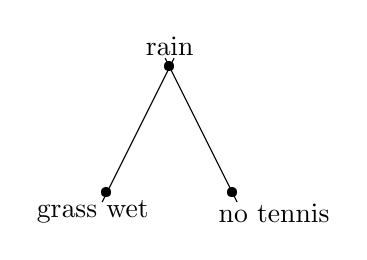
\begin{tikzpicture}[scale=0.8]
		\node[label={[xshift=0em, yshift=-0.5em]\mbox{rain}}] (a) at (1,0) {\textbullet};
		\node[label={[xshift=-0.5em, yshift=-2em]\mbox{grass wet}}, swap] (b) at (0,-2) {\textbullet};
		\node[label={[xshift=1.5em, yshift=-2em]\mbox{no tennis}}, swap] (c) at (2,-2) {\textbullet};
		\draw[-,shorten <=-10pt, shorten >=-10pt] (a) to (b);
		\draw[-,shorten <=-10pt, shorten >=-10pt] (a) to (c);
		\end{tikzpicture}
}}
\end{equation}
}
\cc{两者之间是等价的,起源於 \emp{Stone duality} (every Boolean algebra is isomorphic to a topology of open sets),其后再被推广到 \emp{Priestley} 拓扑对偶 等,都是大同小异的。
}{
	The two are equivalent, originated from \emp{Stone duality} (every Boolean algebra is isomorphic to a topology of open sets), and then generalized to \emp{Priestley} topological duality, etc., all of which are similar .
}

\cc{注意: $\mbox{下雨} \Heytingarrow \mbox{草地湿}$ 是 Heyting implication,这个 $\Heytingarrow$ 的存在 并不是因为「下雨」的\textbf{真值} 比「草地湿」的\textbf{真值 小}。 
}{
	Note: $\mbox{rainy} \Heytingarrow \mbox{grass wet}$ is Heyting implication. The existence of this $\Heytingarrow$ is not because the \textbf{true value} of "rainy" is better than "grass wet"\ textbf{true value is small}.
}

\cc{The Heyting implication $a \Heytingarrow b$ exists for all elements $a, b, x$ such that:
}{
	The Heyting implication $a \Heytingarrow b$ exists for all elements $a, b, x$ such that:
}
\begin{equation}
x \le (a \Heytingarrow b) \quad \mbox{iff} \quad (x \wedge a) \le b.
\end{equation}

\cc{Every Boolean algebra can be a Heyting algebra with the material implication defined as usual: $a \Rightarrow b \equiv \neg a \vee b$.
}{
	Every Boolean algebra can be a Heyting algebra with the material implication defined as usual: $a \Rightarrow b \equiv \neg a \vee b$.
}

\cc{可以用以下例子说明 Heyting implication $\Heytingarrow$ 的定义:
}{
	The following example can be used to illustrate the definition of Heyting implication $\Heytingarrow$:
}
\begin{equation}
\forall X. \quad X \subseteq (\highlight{\mbox{下雨} \Heytingarrow \mbox{草地湿}}) \quad \mbox{iff} \quad (X \wedge \mbox{下雨}) \subseteq \mbox{草地湿}
\end{equation}
\begin{equation}
\vcenter{\hbox{\includegraphics[scale=0.8]{../2020/topology-Heyting-rain-wet.png}}}
\end{equation}

\cc{经典逻辑的 $\Rightarrow$ 和 直觉主义逻辑 $\Heytingarrow$ 只有 在\textbf{边界}上的 微小差异:
}{
	The classic logic $\Rightarrow$ and the intuitive logic $\Heytingarrow$ have only minor differences on the \textbf{boundary}:
}
\begin{align}
\mbox{classical $A \Rightarrow B$} \qquad & \qquad
\mbox{Heyting $A \Heytingarrow B$} \nonumber \\
\vcenter{\hbox{\includegraphics[scale=1]{../2020/topology-classical-implication.png}}}
\qquad & \qquad
\vcenter{\hbox{\includegraphics[scale=1]{../2020/topology-Heyting-implication.png}}}
\end{align}
\cc{无论是何种逻辑,以下的两边是 \textbf{等价}的:
}{
	Regardless of the logic, the following two sides are \textbf{equivalent}:
}
\begin{align}
\mbox{$A \Rightarrow B$} \quad & \Longleftrightarrow \quad \mbox{$A \vdash B$ or $A \subseteq B$} \\
\vcenter{\hbox{\includegraphics[scale=1]{../2020/topology-Heyting-implication.png}}}
\quad & \Longleftrightarrow \quad 
\vcenter{\hbox{\includegraphics[scale=1]{../2020/topology-implication-2.png}}}
\end{align}
\cc{这可以看成是 将白色部分不断 缩小并「消灭掉」的结果。 
}{
	This can be seen as the result of continuously shrinking and "wiping out" the white part.
}

\cc{根据 Stone duality, 既然可以用 Boolean 或 Heyting algebra 做逻辑推导,因此 也可以用 toplogy of (open) sets 做逻辑推导。 其根据的就是:
}{
	According to Stone duality, since Boolean or Heyting algebra can be used for logical derivation, toplogy of (open) sets can also be used for logical derivation. The basis is:
}
\begin{equation}
A \vdash B \quad \mbox{和} \quad A \subseteq B
\end{equation}
\cc{之间的 等价。
}{
	The equivalence between.
}

\cc{这种 topology 可以视为 \textbf{truth table} 的一种形式,如下图所示,每个\textbf{区域}代 表 真值表的\textbf{一行}:
}{
	This kind of topology can be regarded as a form of \textbf{truth table}, as shown in the following figure, each \textbf{area} represents \textbf{line} of the truth table:
}
\begin{equation}
\begin{tabular}{|c|c|c|c|}
\hline 
{\color{red}$A$} & {\color{red}$B$} & {\color{red}$C$} & \# \\ 
\hline 
$\top$ & $\top$ & $\top$ & 1 \\ 
\hline 
$\top$ & $\top$ & $\bot$ & 2 \\ 
\hline 
$\top$ & $\bot$ & $\top$ & 3 \\ 
\hline 
$\top$ & $\bot$ & $\bot$ & 4 \\ 
\hline 
$\bot$ & $\top$ & $\top$ & 5 \\ 
\hline 
$\bot$ & $\top$ & $\bot$ & 6 \\ 
\hline 
$\bot$ & $\bot$ & $\top$ & 7 \\ 
\hline 
$\bot$ & $\bot$ & $\bot$ & 8 \\ 
\hline 
\end{tabular}
\quad \Longleftrightarrow \quad
\vcenter{\hbox{\includegraphics[scale=1]{../2020/topology-ABC.png}}}
\end{equation}

\cc{之所以讲这么多,目的是想说明,Heyting algebra 和我们熟悉的 Boolean algebra 其实有很多共通点。 
}{
	The reason why I have said so much is to explain that Heyting algebra and the familiar Boolean algebra actually have a lot in common.
}

\cc{另一点发现是,在 \S\ref{sec:material-implication} 所说的 material implication 问题,在 intuitionistic logic 里仍然存在。
}{
	Another finding is that the material implication problem mentioned in \S\ref{sec:material-implication} still exists in intuitionistic logic.
}

\cc{In a topos $\mathbb{E}$, the subobject $\mathrm{Sub}_{\mathbb{E}}(A)$ is a \emp{poset} that admits \emp{Heyting implication}.  
}{
	In a topos $\mathbb{E}$, the subobject $\mathrm{Sub}_{\mathbb{E}}(A)$ is a \emp{poset} that admits \emp{Heyting implication}.
}

\cc{Using Kripke semantics, the Heyting arrow $\rightarrow$ can be defined by:
}{
	Using Kripke semantics, the Heyting arrow $\rightarrow$ can be defined by:
}
\begin{equation}
k \Vdash A \rightarrow B \quad \Leftrightarrow \quad \forall \ell \ge k \; (\ell \Vdash A \Rightarrow \ell \Vdash B)
\end{equation}

\cc{Whereas the ``fish-hook'' \emp{strict implication} can be defined as ``A implies B necessarily'':
}{
	Whereas the ``fish-hook'' \emp{strict implication} can be defined as ``A implies B necessarily'':
}
\begin{equation}
A \strictif B \quad \equiv \quad \square (A \Rightarrow B) 
\end{equation}

\cc{The two can be regarded as equivalent via:
}{
	The two can be regarded as equivalent via:
}
\begin{equation}
\begin{aligned}
k \Vdash \square (A \Rightarrow B) \quad \Leftrightarrow \quad & \forall \ell \ge k \; (\ell \Vdash (A \Rightarrow B)) \\
\quad \Leftrightarrow \quad & \forall \ell \ge k \; (\ell \Vdash A \Rightarrow \ell \Vdash B)
\end{aligned}
\end{equation}

\cc{问题是将 Heyting implication 定义 by possible worlds semantics 有什么好处?  从 machine learning 角度可能更合理。  但其实也好像包含 classical implication 所以是循环的?  
}{
	The question is what are the benefits of defining Heyting implication by possible worlds semantics? It may be more reasonable from the perspective of machine learning. But in fact, it also seems to contain classical implication, so it is cyclic?
}

\cc{根据 topos 理论,Heyting implication 的出现是因为 sub-objects 的 Heyting algebra.  但我希望 implication arrow 纯粹是因为 BHK interpretation 而出现的。 
}{
	According to topos theory, Heyting implication appears because of Heyting algebra of sub-objects. But I hope implication arrow appears purely because of BHK interpretation.
}

\cc{Heyting implication 的问题是它产生自 sub-object 概念。 Material truth will cause an implication to exist.  What does that mean?  
}{
	The problem with Heyting implication is that it arises from the concept of sub-object. Material truth will cause an implication to exist. What does that mean?
}
	
\section{Modal logic}

\cc{Modalities are often conceived in terms of variation over some collection or \textbf{possible worlds}.
}{
	Modalities are often conceived in terms of variation over some collection or \textbf{possible worlds}.
}

\cc{A modal operator (such as $\square$) in the category $\mathbf{Sheaf}(X)$ is a \emp{sheaf morphism} $\square: \Omega \rightarrow \Omega$ satisfying 3 conditions, $\forall U \subseteq X$ and $p, q \in \Omega(U)$:
}{
	A modal operator (such as $\square$) in the category $\mathbf{Sheaf}(X)$ is a \emp{sheaf morphism} $\square: \Omega \rightarrow \Omega$ satisfying 3 conditions, $\forall U \subseteq X$ and $p, q \in \Omega(U)$:
}
\begin{equation}
\begin{aligned}
& \mbox{a)} \quad p \le \square (p) \\
& \mbox{b)} \quad (\square ; \square) (p) \le \square (p) \\
& \mbox{c)} \quad \square (p \wedge q) = \square (p) \wedge \square (q)
\end{aligned}
\end{equation}

\subsection{Possible-world semantics}

\cc{Possible-world semantics is also called \emp{intensional semantics}, as opposed to \emp{extensional semantics} where truth values are directly assigned to propositions.  Does this idea jibe with the other definition of ``intension'', ie, as opposed to Leibniz extensionality and also related to intensional logic?
}{
	Possible-world semantics is also called \emp{intensional semantics}, as opposed to \emp{extensional semantics} where truth values are directly assigned to propositions.  Does this idea jibe with the other definition of ``intension'', ie, as opposed to Leibniz extensionality and also related to intensional logic?
}

\begin{equation}
\nonumber
\mbox{Saul Kripke (1940-)} \quad 
\vcenter{\hbox{\includegraphics[scale=0.5]{../2020/Kripke.jpg}}}
\end{equation}

\subsection{Computer implementation of possible worlds}

\cc{要詮釋 modal logic,需要引入 frame $F = \langle W, R, D, H \rangle$, 其中:
}{
	To interpret modal logic, you need to introduce frame $F = \langle W, R, D, H \rangle$, where:
}
\begin{itemize}
	\cc{	\item $W$ = set of possible worlds = $\{ w_1, w_2, ... \}$
	}{
		\item $W$ = set of possible worlds = $\{ w_1, w_2, ... \}$
	}
	\cc{	\item $R$ = a relation between worlds, $w_i R w_j$
	}{
		\item $R$ = a relation between worlds, $w_i R w_j$
	}
	\cc{	\item $D$ = domain of first-order objects
	}{
		\item $D$ = domain of first-order objects
	}
	\cc{	\item $H: W \rightarrow \powerset(D)$, for each world specify a subset of objects
	}{
		\item $H: W \rightarrow \powerset(D)$, for each world specify a subset of objects
	}
\end{itemize}

\cc{To interpret formulas with $\square$:
}{
	To interpret formulas with $\square$:
}
\begin{equation}
M \Vdash \square A \; [w] \quad \Leftrightarrow \quad \forall w' \succeq w. \; M \Vdash A \; [w']
\end{equation}
\cc{這牽涉到要 quantify over all $w$'s.
}{
	This involves quantify over all $w$'s.
}

\cc{重點是 inference 需要什麼 data?
}{
	The point is what data does inference need?
}

\cc{顯然需要決定在某 $w$ 中 $p$ 是否成立,甚至需要判斷 $\forall w. p [w]$.
}{
	Obviously it is necessary to decide whether $p$ is established in a certain $w$, and even to judge $\forall w. p [w]$.
}

\cc{後者似乎需要將所有 有關的可能世界(或至少是其 summary)放到 working memory 再 quantify.  
}{
	The latter seems to need to put all relevant possible worlds (or at least their summary) into working memory and then quantify.
}

\subsection{Intensional vs extensional}

``Beethoven's 9th symphony'' and ``Beethoven's choral symphony'' have the same \emp{extension} but different \emp{intensions}.

\subsection{Intensional logic}

\cc{Possible-world semantics is also called \emp{intensional semantics}, as opposed to \emp{extensional semantics} where truth values are directly assigned to propositions.
}{
	Possible-world semantics is also called \emp{intensional semantics}, as opposed to \emp{extensional semantics} where truth values are directly assigned to propositions.
}

\cc{Logic terms differ in intension if and only if it is \textbf{possible} for them to differ in extension.  Thus, \emp{intensional logic} interpret its terms using possible-world semantics.
}{
	Logic terms differ in intension if and only if it is \textbf{possible} for them to differ in extension.  Thus, \emp{intensional logic} interpret its terms using possible-world semantics.
}

\subsection{Strict implication}
\label{sec:strict-implication}

\subsubsection{The problem of ``material implication''}

\cc{Material implication 的意思是「实质蕴涵」,亦即是说 $A \Rightarrow B$ 等价於 $\neg A \vee B$,其真值表如下:
}{
	Material implication means "substantial implication", which means that $A \Rightarrow B$ is equivalent to $\neg A \vee B$, and its truth table is as follows:
}

\begin{equation}
\label{eqn:implication-truth-table}
\begin{tabular}{|c|c|c|}
\hline 
$A$ & $B$ & $A \Rightarrow B$ \\ 
\hline \hline 
0 & 0 & 1 \\
\hline 
0 & 1 & 1 \\ 
\hline 
1 & 0 & 0 \\ 
\hline 
1 & 1 & 1 \\ 
\hline 
\end{tabular} 
\end{equation}

\cc{Material implication 的概念向来很有争议,例如,当前提是错误时,它永远是真的: 
}{
	The concept of material implication has always been controversial. For example, when the current mention is wrong, it is always true:
}
\begin{equation}
\mbox{瑞士在非洲} \Rightarrow \mbox{猪会飞}
\end{equation}

\begin{center}
	\rule{0.8\textwidth}{1pt}
\end{center}

\cc{透过观察 truth table 可以发现,它的每一列 其实代表一个 \emp{可能世界},这些 可能世界 是不会 同时发生的。 换句话说,material implication 和 strict implication 本来是一样的,只是前者将 可能世界 的语义 隐蔽到「幕后」。 
}{
	By observing the truth table, we can find that each column of it actually represents a \emp{possible world}, and these possible worlds will not happen at the same time. In other words, material implication and strict implication are originally the same, but the former hides the semantics of the possible world "behind the scenes."
}

\cc{For strict implication to make sense, it is always necessary to invoke possible-world semantics.  A strict implication is always \emp{learned} from numerous examples from experience, in accord with the philosophical tradition of ``empiricism''.
}{
	For strict implication to make sense, it is always necessary to invoke possible-world semantics.  A strict implication is always \emp{learned} from numerous examples from experience, in accord with the philosophical tradition of ``empiricism''.
}

\cc{Strict implication is equivalent to material implication over multiple instances.  The truth table of material implication agrees with the functional interpretation of implication.  
}{
	Strict implication is equivalent to material implication over multiple instances.  The truth table of material implication agrees with the functional interpretation of implication.
}

{\color{red}
	\begin{center}
		\rule{0.8\textwidth}{1pt} \\
		\cc{
		以下部分 包含很多未落实的想法,包括我自己的 ``thinking aloud'' }{
		The following section contains many unimplemented ideas, including my own ``thinking aloud''
		}
	\end{center}
}

\section{Fuzzy logic}
\label{sec:fuzzy-logic}

\begin{equation}
\nonumber
\parbox{7cm}{
	\mbox{Lotfi Zadeh (1921-2017)} \\
	\mbox{[Iranian-Jewish]}} \qquad 
\vcenter{\hbox{\includegraphics[scale=2.5]{../2020/Zadeh.jpg}}}
\end{equation}

\cc{举例来说,「人」的概念由若干个 \emp{属性} (properties) 表示:
}{
	For example, the concept of "person" is represented by several \emp{properties} (properties):
}
\begin{equation}
\vcenter{\hbox{\includegraphics[scale=0.7]{../2020/properties-of-human.png}}}
\end{equation}
\cc{例如说: 人是动物的一种、人有智慧、人有某些感情、人有某些道德观念、等。 这些属性是「人」这个概念的 \emp{intension}.  但「人」这个概念的 \emp{extension} 是这个 \textbf{集合}的\textbf{元素},例如 John, Mary 等。
}{
	For example, humans are a kind of animals, humans have wisdom, humans have certain emotions, humans have certain moral concepts, etc. These attributes are the \emp{intension} of the concept of "person". But the \emp{extension} of the concept of "person" is the \textbf{element} of this \textbf{set}, such as John, Mary, etc.
}

\cc{而「John」的属性是更为 \textbf{特殊} (specific) 的:
}{
	And the attribute of "John" is more \textbf{special} (specific):
}
\begin{equation}
\vcenter{\hbox{\includegraphics[scale=0.7]{../2020/properties-of-John.png}}}
\end{equation}
\cc{问题是怎样决定 \ ``{\color{red} John} is {\color{blue}human}'' = {\color{blue}human}({\color{red}john}) 这个命题的 fuzzy truth value.
}{
	The problem is how to decide \ ``{\color{red} John} is {\color{blue}human}'' = {\color{blue}human}({\color{red}john}) The fuzzy truth of this proposition value.
}

\cc{或者用一个男人更容易明白的例子: 当我们说「玛丽莲梦露 很性感」,这个命题的 fuzzy truth value 就是「Marilyn 的属性」和「性感的属性」之间的某种 \textbf{共同性}的量度。  这种 truth value 的定义 是基於 \textbf{intension} 而不是 extension.
}{
	Or use an example that is easier for a man to understand: When we say "Marilyn Monroe is sexy", the fuzzy truth value of this proposition is a certain \textbf{commonality between "Marilyn's attributes" and "sexy attributes" } Measurement. This definition of truth value is based on \textbf(intension) rather than extension.
}

\cc{但 dually,用 \textbf{extension} 的角度定义 truth value 也未尝不可:
}{
	But dually, it is not impossible to define the truth value from the perspective of \textbf{extension}:
}
\begin{itemize}
	\cc{	\setlength{\itemsep}{0.1ex}  % this works locally
	}{
		\setlength{\itemsep}{0.1ex}  % this works locally
	}
	\cc{	\item 每个 fuzzy proposition 看成是一个 set, 里面有 该命题的「证明」
	}{
		\item Each fuzzy proposition is regarded as a set, which contains the ``proof'' of the proposition
	}
	\cc{	\item 例如「人类」的集合是「有人类」这个命题的证明
	}{
		\item For example, the set of "human beings" is a proof of the proposition that "there are human beings"
	}
	\cc{	\item 而,「数学家」作为「人类」的子集,等於命题「所有人都是数学家」的证明
	}{
		\item And, "mathematician" as a subset of "human beings" is equivalent to the proof of the proposition "Everyone is a mathematician"
	}
\end{itemize}
\cc{但在某些情况下,``A is B'' 但 $A$ 不是\textbf{集合}(例如 John 或 Marilyn 不是集合),则 extensional 的诠释 不适用。 
}{
	But in some cases, ``A is B'' but $A$ is not a \textbf{set} (for example, John or Marilyn is not a set), the interpretation of extensional does not apply.
}

\cc{无论 intensional 或 extensional, 这种诠释方法 跟 HoTT 理论 (\S\ref{sec:HoTT}) 是融洽的: 概念「John」的 \textbf{证明} 是 $J_1 \wedge J_2 ... \wedge J_n \Rightarrow$ John, 其中 $J_i$ 是 John 的 \textbf{属性}。  同理,「handsome」的证明是 $H_1 \wedge H_2 ... \wedge H_n \Rightarrow$ handsome.  因此 ``John is handsome`` 的 fuzzy truth value 是 $\{ J_i \}$ 和 $\{ H_i \}$ 的共通性(例如交集或并集)的某种量度。
}{
	Regardless of intensional or extensional, this interpretation method is in harmony with HoTT theory (\S\ref{sec:HoTT}): the \textbf{proof} of the concept "John" is $J_1 \wedge J_2 ... \wedge J_n \Rightarrow$ John, where $J_i$ is John’s \textbf{attribute}. Similarly, the proof of "handsome" is $H_1 \wedge H_2 ... \wedge H_n \Rightarrow$ handsome. Therefore, the fuzzy truth value of ``John is handsome'' is a measure of the commonality (such as intersection or union) of $\{ J_i \}$ and $\{ H_i \}$.
}

\cc{关於 fuzzy truth value 还有个问题: 一个对象的 \textbf{属性} 在某程度上可以随意增加或减少,因此纯粹 计算 属性的\textbf{数量},并不能客观地决定 truth value.  似乎每个 属性 应该有某种 \emp{测度} (measure) 或 \emp{权重} (weight), 这样在改变 属性 的描述时,fuzzy truth value 保持\textbf{不变}。
}{
	There is another problem with the fuzzy truth value: The \textbf{attribute} of an object can be increased or decreased at will to a certain extent, so purely calculating the \textbf{number} of the attribute cannot objectively determine the truth value. It seems that each attribute There should be some kind of \emp{measure} (measure) or \emp{weight} (weight), so that when the description of the attribute is changed, the fuzzy truth value remains \textbf{unchanged}.
}

\cc{问题是 witness 是什么?  例如「匙羹在杯内」是因为其他 视觉 propositions 得到的结论。 它是 true 这一点是重要的,但它的 ``intension'' 更重要。  或者说 proof 过程中处理的是 proof objects.  
}{
	What is a proof witness?  For example, ``the spoon is in the cup'' is the result of other visual propositions.  Its truth is important, but its ``intension'' is even more important.  In other words, proof objects are the essence in the proof process.
}

\cc{这个 proof object 它除了是一件 syntactic 的东西之外还可以是什么?  或者说 map 的 \textbf{domain} 是命题,但被 map 映射的是 evidence?
}{
	What can this proof object be besides being a syntactic thing? In other words, the \textbf{domain} of the map is a proposition, but what is mapped by the map is evidence?
}

\subsection{Fuzzy implication}
\label{sec:fuzzy-implication}

\cc{本节 考察一下 fuzzy implication $A \stackrel{\sim}{\Rightarrow} B$ 的真值是如何确定的?  在  \S\ref{sec:material-implication} 已经分析过 经典 material implication 的性质。
}{
	This section examines how the true value of fuzzy implication $A \stackrel{\sim}{\Rightarrow} B$ is determined? The properties of classic material implication have been analyzed in \S\ref{sec:material-implication}.
}

\cc{From above analysis, material implication seems to be a statistical result.  Some cases cause the implication to be true, some cases cause it to be false.  Overall, it's truth value would have to be consistent with \textbf{all} cases;  which (under binary logic) is feasible.
}{
	From above analysis, material implication seems to be a statistical result.  Some cases cause the implication to be true, some cases cause it to be false.  Overall, it's truth value would have to be consistent with \textbf{all} cases;  which (under binary logic) is feasible.
}

\cc{So, is this saying that the TV of (binary) implication is statistically determined?  If so, can we just do the same for fuzzy implication?  Sure, why not?
}{
	So, is this saying that the TV of (binary) implication is statistically determined?  If so, can we just do the same for fuzzy implication?  Sure, why not?
}

\cc{But then do we still have a ``truth table'' of fuzzy implication?  What exactly is a ``truth table'', anyway?
}{
	But then do we still have a ``truth table'' of fuzzy implication?  What exactly is a ``truth table'', anyway?
}

\cc{If $A \stackrel{\sim}{\Rightarrow} B$ is a proposition, then what are its \textbf{proofs}?  This should be interpreted as ``the number of maps from $A$ to $B$''.  关键是利用这一点来定义 fuzzy implication 的 truth value.
}{
	If $A \stackrel{\sim}{\Rightarrow} B$ is a proposition, then what are its \textbf{proofs}? This should be interpreted as ``the number of maps from $A$ to $B$'' The key is to use this to define the truth value of fuzzy implication.
}

\cc{Fuzzy truth values arise from imperfect proofs.  Fuzzy implication arises from maps between imperfect proofs.  Why does a map between proofs become less than 1?  
}{
	Fuzzy truth values arise from imperfect proofs.  Fuzzy implication arises from maps between imperfect proofs.  Why does a map between proofs become less than 1?
}

\cc{首先,number of maps 其实都有问题。  根据 fuzzy intension, 其实不是 number of proofs 而是 proof 的 imperfect.  The measure of whether one proof is a subset of another proof.  This forms the basis of a ``predication'' proposition.  But what if the proposition is an implicational one?  Then it would be a map from the proof of one proposition to the proof of another.
}{
	首先,number of maps 其实都有问题。  根据 fuzzy intension, 其实不是 number of proofs 而是 proof 的 imperfect.  The measure of whether one proof is a subset of another proof.  This forms the basis of a ``predication'' proposition.  But what if the proposition is an implicational one?  Then it would be a map from the proof of one proposition to the proof of another.
}

\cc{Rethink the binary case.  There exist (or not) proofs of A, B.  From which we establish a map from proof of A to proof of B.  But when the proof of A is empty then there could be no such map.  The truth value of the implication statement must somehow be \textbf{consistent} with the \textbf{existence} of such maps.  So there is a case where such a map is impossible and thus the implication would be false.
}{
	Rethink the binary case.  There exist (or not) proofs of A, B.  From which we establish a map from proof of A to proof of B.  But when the proof of A is empty then there could be no such map.  The truth value of the implication statement must somehow be \textbf{consistent} with the \textbf{existence} of such maps.  So there is a case where such a map is impossible and thus the implication would be false.
}

\cc{如果 A 的 proof fuzzy 到几乎唔存在,(而B的proof is true),咁 $A \Rightarrow B$ 的 fuzzy TV 是不是应该接近 false?  Well, there is the possibility of probabilistic.  Suppose we assume that it is deterministic but fuzzy.  Then the above requirement is clearly correct (if we just think of a simple example).  So the fuzzy implication's TV is just a generalization of the binary \textbf{truth table}.
}{
	If A's proof fuzzy 到几乎唔存在,(but B's proof is true), then $A \Rightarrow B$ 的 fuzzy TV 是不是应该接近 false?  Well, there is the possibility of probabilistic.  Suppose we assume that it is deterministic but fuzzy.  Then the above requirement is clearly correct (if we just think of a simple example).  So the fuzzy implication's TV is just a generalization of the binary \textbf{truth table}.
}

\cc{But how can we interpret the fuzzy implication's TV as a measure (perhaps the cardinality) of its \textbf{map}?  According to the binary view, it is a measure of the existence of maps between A and B.  In which case, a weak proof of A means that the map from A to B would be weak also.
}{
	But how can we interpret the fuzzy implication's TV as a measure (perhaps the cardinality) of its \textbf{map}?  According to the binary view, it is a measure of the existence of maps between A and B.  In which case, a weak proof of A means that the map from A to B would be weak also.
}

\cc{Looking at the following table from a ``conditional'' view, it seems reasonable:
}{
	Looking at the following table from a ``conditional'' view, it seems reasonable:
}
\begin{equation}
\begin{tabular}{|c|c|c|c|}
\hline 
$A$ & $B$ & $A \stackrel{\sim}{\Rightarrow} B$ & $B^A$ \\ 
\hline \hline 
\mbox{weak} & \mbox{weak} & \mbox{strong} & $0^0 = 1$ \\
\hline 
\mbox{weak} & \mbox{strong} & \mbox{strong} & $1^0 = 1$ \\ 
\hline 
\mbox{strong} & \mbox{weak} & \mbox{weak} & $0^1 = 0$ \\ 
\hline 
\mbox{strong} & \mbox{strong} & \mbox{strong} & $1^1 = 1$ \\ 
\hline 
\end{tabular} 
\end{equation}
\cc{but the problem is how to interpret the truth value of $A \stackrel{\sim}{\Rightarrow} B$ as \textbf{counting} the number of maps?
}{
	but the problem is how to interpret the truth value of $A \stackrel{\sim}{\Rightarrow} B$ as \textbf{counting} the number of maps?
}

subsection{Fuzzy functions?}

\cc{What are fuzzy functions?  \underconst
}{
	What are fuzzy functions?  \underconst
}

\section{Homotopy type theory (HoTT)}
\label{sec:HoTT}

\begin{equation}
\nonumber
\mbox{Vladimir Voevodsky (1966-2017)} \quad 
\vcenter{\hbox{\includegraphics[scale=0.25]{../2020/Voevodsky.jpg}}}
\end{equation}

\cc{HoTT 的中心思想是将 types 看成是某些 空间 (spaces),而这些空间可以被赋予 topological 特别是 homotopy 结构。 在 homotopy 而言,关键是 将 type $A$ 里面两个元素的 \textbf{相等} $\mathrm{id}_A$ 看成是 homotopy 的 \textbf{path}.
}{
	The central idea of HoTT is to regard types as certain spaces, and these spaces can be given topological, especially homotopy structures. In terms of homotopy, the key is to treat the \textbf{equal} $\mathrm{id}_A$ of the two elements in type $A$ as the \textbf{path} of homotopy.
}

\subsection{Why HoTT may be useful}

\cc{在 topos 上 $A \subseteq B$ 或 $a \in A$ 是一种 subset 关系,或者可以说是 topological 关系。  在计算机上,将这个 topology 赋予更多「空间」的特性,例如 vector space, metric space 等,似乎会是很 powerful 的。 
}{
	On topos, $A \subseteq B$ or $a \in A$ is a subset relationship, or it can be said to be a topological relationship. On the computer, giving this topology more "space" features, such as vector space, metric space, etc., seems to be very powerful.
}

\cc{但问题是: 如果 $A$ 是 拓扑空间中某个(形状已知的)region,而 entity $a$ 的位置也是知道的,则 $a \in A$ 这个命题的真假 也立即可以知道。 但这是非常有问题的,例如「$e \in?$ 无理数」这个命题,必需复杂的证明,而不是瞬间可以判断。 又或者「OJ Simpson $\in?$ 杀人凶手」。
}{
	But the problem is: if $A$ is a region (with known shape) in topological space, and the position of entity $a$ is also known, then the true or false of the proposition $a \in A$ can also be known immediately. But this is very problematic. For example, the proposition "$e \in?$ irrational number" requires complex proofs, not instant judgments. Or "OJ Simpson $\in?$ Murderer".
}

\cc{换句话说,似乎不可能将 命题空间 实现成某种有 \textbf{具体位置}的空间。  因此 $a \in A$ 这种命题,似乎 只能够表述成 ordered pair $(a, A)$,然后用\textbf{代数方法} 模拟 abstract topology.  这 其实就是我在 (\ref{eqn:brutal-syntactic-method}) 提到的「粗暴」syntactic 方法。 
}{
	In other words, it seems impossible to realize the propositional space into a space with \textbf{specific location}. Therefore, the proposition $a \in A$ can only be expressed as an ordered pair $(a, A)$, and then use \textbf{algebraic method} to simulate abstract topology. This is actually what I am in (\ref{eqn:brutal -syntactic-method}) The "crude" syntactic method mentioned.
}

\cc{挽救「位置空间」的一个办法是: 容许 OJ Simpson $\in$「黑人、男性、演员、球员」等,但保证他不属於其他(未被验证的)集合,后者是\textbf{未知}的。 但这样导致要 验证 潜在无穷多个集合,并不可行。
}{
	One way to save the "location space" is to allow OJ Simpson $\in$ "blacks, men, actors, players", etc., but ensure that he does not belong to other (unverified) collections, the latter is \textbf{unknown} of. But this leads to the verification of potentially infinite sets, which is not feasible.
}

\cc{除非在 逻辑空间中 预先保证 每个集合 \textbf{并不相交},而如果 $x \in A \; \wedge \; x \in B$,则 设定 $x_1 \in A, \; x_2 \in B, \; x_1 = x_2$, and $x_1, x_2$ are \textbf{path-connected}.  所以这需要用到 HoTT.
}{
	Unless in the logical space, each set \textbf{does not intersect} is guaranteed in advance, and if $x \in A \; \wedge \; x \in B$, set $x_1 \in A, \; x_2 \ in B, \; x_1 = x_2$, and $x_1, x_2$ are \textbf{path-connected}. So this requires HoTT.
}

\cc{暂时 仍未知道 这种做法 是不是比「粗暴」法更有效率。 
}{
	It is not yet known whether this approach is more efficient than the "crude" approach.
}

\cc{根据 paths 可以有如下的 topological「变形」:
}{
	According to paths, there can be the following topological "deformations":
}
\begin{equation}
\vcenter{\hbox{\includegraphics[scale=0.9]{../2020/path-morphing-1.png}}}
\quad \Longleftrightarrow \quad
\vcenter{\hbox{\includegraphics[scale=0.9]{../2020/path-morphing-2.png}}}
\end{equation}
\cc{但右边 仍是会出现 $x \in A$ accidentally 导致 $x \in B$ 的情况。
}{
	But on the right, there will still be a situation where $x \in A$ accidentally causes $x \in B$.
}

\cc{如果 neural network map $F$ 的对象不是 ordered pairs ($x \in A$), 可以是什么?  A \textbf{proposition} can be regarded as a set of points $x_i$ connected by paths.  
}{
	If the object of neural network map $F$ is not ordered pairs ($x \in A$), what can it be? A \textbf{proposition} can be regarded as a set of points $x_i$ connected by paths.
}

\subsection{HoTT levels}

\begin{equation}
\begin{tabular}{|c|c|}
... & ... \\ 
\hline 
2 & 2-groupoids \\ 
\hline 
1 & groupoids \\ 
\hline 
0 & sets \\ 
\hline 
-1 & (mere) propositions \\ 
\hline 
-2 & contractable spaces \\ 
\hline 
\end{tabular} 
\end{equation}

\subsubsection{Truncation}

\cc{$||A||$ is a way to obtain the \textbf{truth value} of a type $A$, known as \textbf{truncation}.  For Voevodsky, the truth value is always binary, the type of ``mere propositions''.  I propose that it can be generalized such that, on HoTT level 0, it provides the \textbf{fuzzy} truth value $\in [0,1]$.
}{
	$||A||$ is a way to obtain the \textbf{truth value} of a type $A$, known as \textbf{truncation}.  For Voevodsky, the truth value is always binary, the type of ``mere propositions''.  I propose that it can be generalized such that, on HoTT level 0, it provides the \textbf{fuzzy} truth value $\in [0,1]$.
}

\subsection{What is homotopy?}

\subsection{Univalence axiom}

\cc{在 HoTT 的 set 的层次,``='' 是一个 predicate, 根据我的理论可以看成是 fuzzy predicate.
}{
	At the set level of HoTT, ``='' is a predicate, which can be regarded as a fuzzy predicate according to my theory.
}

\cc{如果我没理解错误,univalence axiom 的意思 似乎是将 = 的 fuzzy truth value「强制」成 binary.
}{
	If I did not understand the error, the meaning of univalence axiom seems to be to "force" the fuzzy truth value of = into binary.
}

\section{Transfer to deep learning}

\cc{这一节讨论 如何将上面提到的 logic structure 转移到 深度学习的 神经网络 (neural network, NN)。  一般来说,很难将 额外的结构 impose 在 神经网络上,因为 NN 本身已经有很 ``rigid'' 的结构。 在这方向上成功的例子是 CNN (convolutional NN),其中 convolution $f * g$ 是由 ``weight sharing'' 模拟。 但除此之外,一般很难在 NN 上添加结构。
}{
	This section discusses how to transfer the logic structure mentioned above to the neural network (NN) of deep learning. Generally speaking, it is difficult to impose additional structures on the neural network, because the NN itself already has a very ``rigid'' structure. A successful example in this direction is CNN (convolutional NN), where convolution $f * g$ is simulated by ``weight sharing''. But other than that, it is generally difficult to add structure to the NN.
}

\emp{Symmetric NN} 是一种 在输入变量的 \textbf{置换}下 不变 (permutation invariant) 的神经网络。 其解决 办法 是利用以下的 函数形式:
\begin{equation}
f(x_1, ..., x_n) = g(h(x_1) + ... + h(x_n))
\end{equation}
\begin{equation}
\vcenter{\hbox{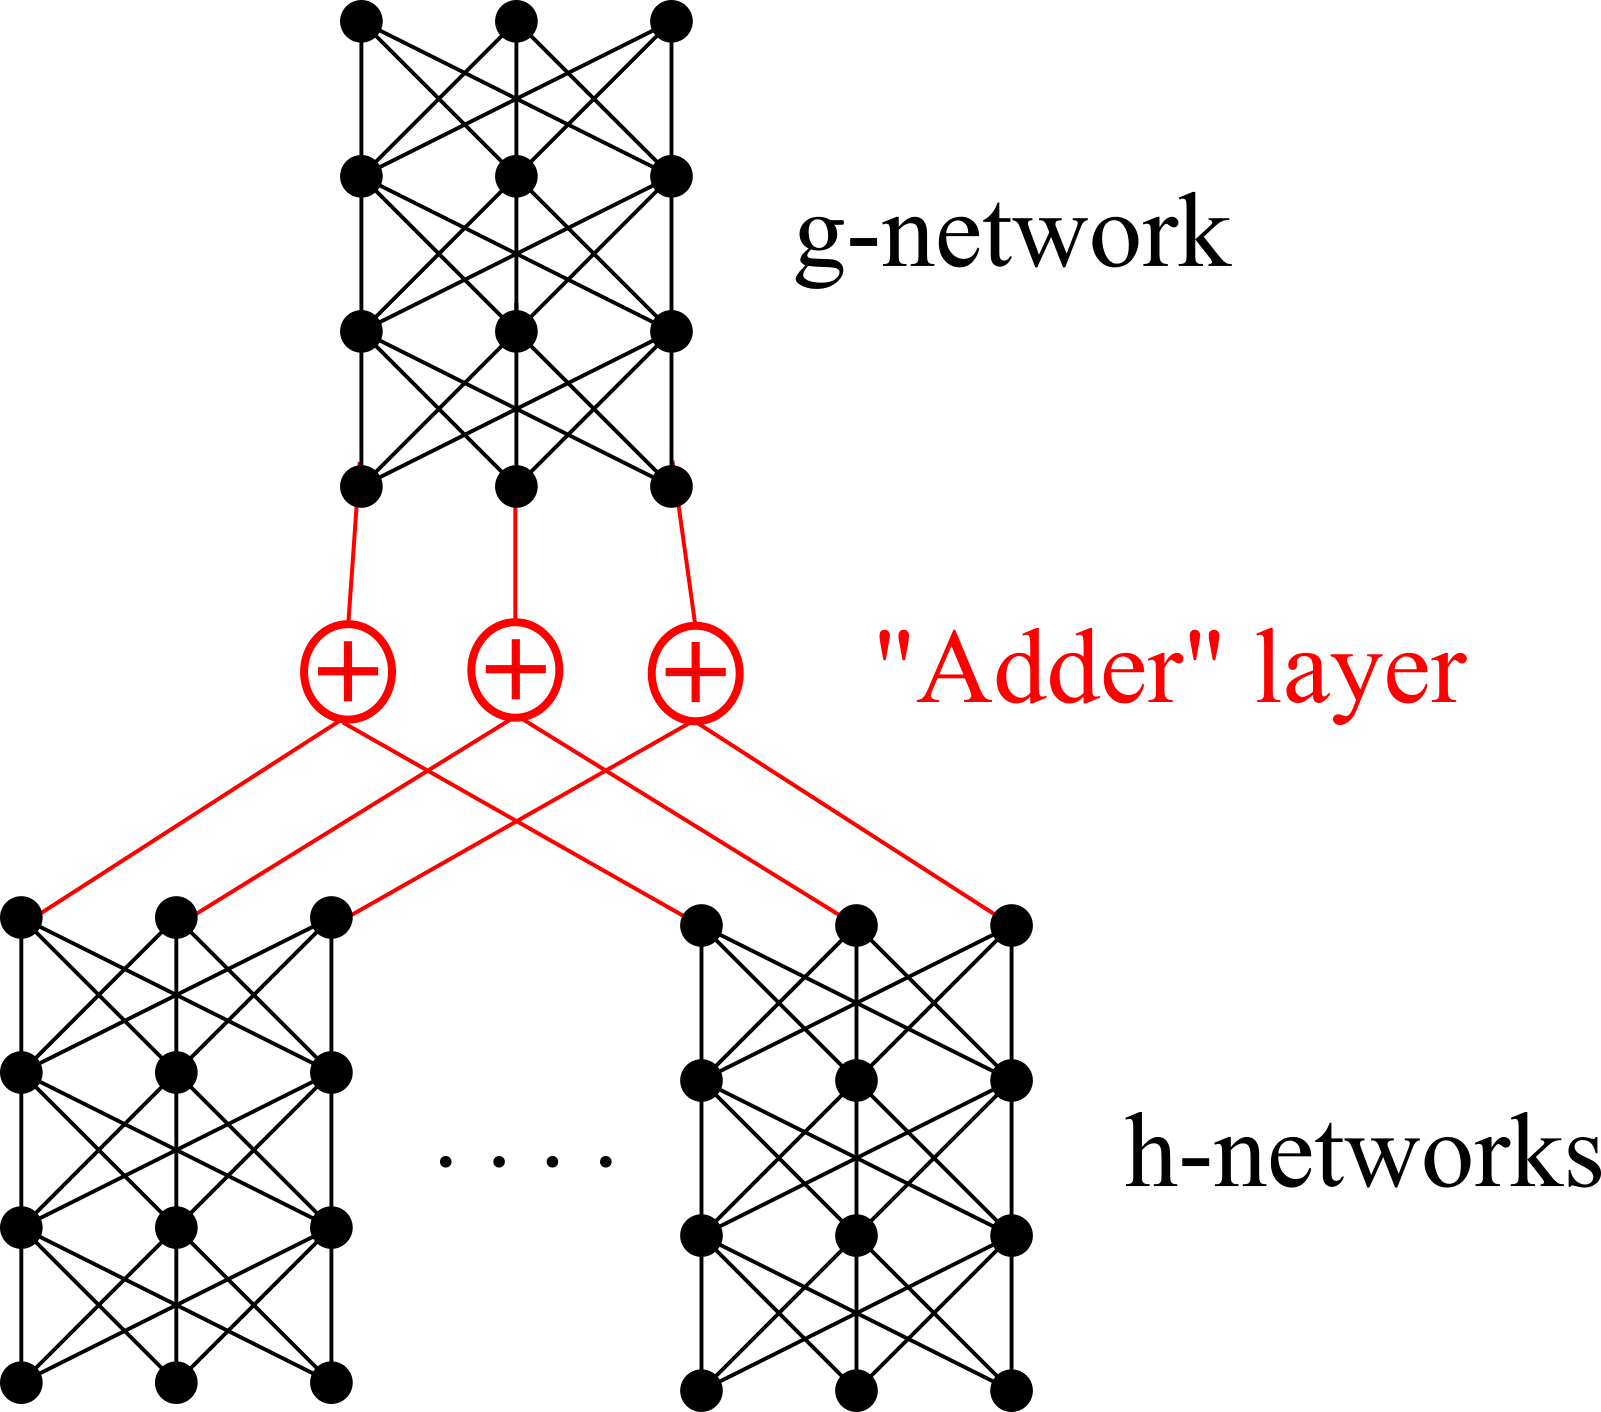
\includegraphics[scale=0.5]{../2020/g-and-h-networks.png}}}
\end{equation}
\cc{注意在这个方案下,NN 是以 ``black box'' 作为 building blocks; 内部结构不变。 
}{
	Note that under this scheme, NN uses ``black box'' as building blocks; the internal structure remains unchanged.
}

\cc{范畴论 的好处是,将一切用 morphisms, compositions, pullbacks, adjunctions, 等 表示; 这种做法 很容易用 NN implement.
}{
	The advantage of category theory is that everything is represented by morphisms, compositions, pullbacks, adjunctions, etc.; this approach is easy to implement with NN.
}

\subsection{Propositional aspect}

\cc{在命题逻辑的层次上,我选择了最简单的特性,亦即是命题之间的 commutativity:
}{
	At the level of propositional logic, I chose the simplest characteristic, which is commutativity between propositions:
}
\begin{equation}
\begin{aligned}
A &\wedge B & \equiv && B & \wedge A \\
\mbox{\cc{下雨}{it's raining}} &\wedge \mbox{\cc{失恋}{lovesick}} & \equiv && \mbox{\cc{失恋}{lovesick}} &\wedge \mbox{\cc{下雨}{it's raining}}
\end{aligned}
\end{equation}
\cc{但我没有 fully exploit Heyting algebra or Boolean algebra 的结构,因为可以预见 将来是会 推广到 fuzzy-probabilistic logic,而后者的结构只需要 $\wedge$ 和 $\Rightarrow$,和 binary logic 有些不同(迟些解释....)
}{
	But I did not fully exploit the structure of Heyting algebra or Boolean algebra, because it is foreseeable that it will be extended to fuzzy-probabilistic logic in the future, and the latter structure only requires $\wedge$ and $\Rightarrow$, which is slightly different from binary logic (later Explanation....)
}

\subsection{Predicate aspect}

\cc{目前,一般的深度学习模型是比较 简单/粗暴 地作用在 自然语言句子的 \textbf{syntax} 层面,例如: 
}{
	At present, the general deep learning model is relatively simple/crudely applied to the \textbf{syntax} level of natural language sentences, for example:
}
\begin{equation}
\label{eqn:brutal-syntactic-method}
\mbox{``Je {\small\textbullet}
	suis {\small\textbullet}
	\'{e}tudiant'' } \stackrel{f}{\Longrightarrow} \mbox{``I {\small\textbullet}
	am {\small\textbullet}
	student''}
\end{equation}
\cc{句子中的 words 是用 \textbf{Word2Vec} 方式 embed 到向量空间。 但如果用了 Curry-Howard 对应,则会有些微不同,而这个微妙的差异 在数学上比较完美,实际上 computer implementation 会不会比较优胜? 再看一次 Curry-Howard correspondence:
}{
	The words in the sentence are embed into the vector space in the way of \textbf{Word2Vec}. But if Curry-Howard is used, there will be a slight difference, and this subtle difference is mathematically perfect. In fact, will the computer implementation be better? Look again at Curry-Howard correspondence:
}
\begin{equation}
\tag{\ref{eqn:Curry-Howard}}
\begin{aligned}
\underdash{$A \Longrightarrow B$} & \\
\witness \; \stackrel{f}{\longmapsto} \; \witness \hspace*{10pt} &
\end{aligned}
\end{equation}
\cc{这里 $A$ 和 $B$ 是\textbf{逻辑命题},例如「我是学生」; $f$ 将 $A$命题里面的 witness $\witness$ 映射到$B$命题里面。 注意:「我是学生」这些\textbf{语法}上的信息,是以 $f$ 的 \emp{domain} 和 \emp{co-domain} 表示的。 
}{
	Here $A$ and $B$ are \textbf{logic propositions}, such as "I am a student"; $f$ maps the witness $\witness$ in the $A$ proposition to the $B$ proposition. Note: The information on the \textbf{syntax} of "I am a student" is represented by the \emp{domain} and \emp{co-domain} of $f$.
}

\cc{这一节 我们要讨论的是 命题及其内部 在计算机上的 implementation 问题。 再看一次 图 (\ref{eqn:2-levels-of-TT}) 的 两个层次:
}{
	In this section, we are going to discuss the proposition and its internal implementation on the computer. Look again at the two levels in the picture (\ref{eqn:2-levels-of-TT}):
}
\begin{equation}
\tag{\ref{eqn:2-levels-of-TT}}
\vcenter{\hbox{\includegraphics[scale=0.8]{../2020/why-Martin-Lof.png}}}
\end{equation}
\cc{{\color{red}红色 $\rightarrow$} 是 \textbf{predicates} 形成的层次。 $A$ 和 $B$ 是两个不同的\textbf{空间}。 在 $A$ \textbf{内部},Socrates 也是一个空间,Human 是另一个空间,而 Human(Socrates) 构成新的空间(透过 dependent type constructor $\Sigma$)。 
}{
	{\color{red}red $\rightarrow$} is the level formed by \textbf{predicates}. $A$ and $B$ are two different \textbf{spaces}. In $A$ \textbf{inside}, Socrates is also a space, Human is another space, and Human(Socrates) constitutes a new space (through dependent type constructor $\Sigma$).
}

\cc{假设 $X \in \mathcal{U}_1, P \in \mathcal{U}_2, P(X) \in \mathcal{U}_3$,(这些 $\mathcal{U}_i$ 是 type universes), 在计算机上最简单的做法是令:
}{
	Suppose $X \in \mathcal{U}_1, P \in \mathcal{U}_2, P(X) \in \mathcal{U}_3$, (these $\mathcal{U}_i$ are type universes) , The easiest way on the computer is to:
}
\begin{equation}
\mathcal{U}_3 = \mathcal{U}_1 \times \mathcal{U}_2
\end{equation}
\cc{这和 \S\ref{sec:Martin-Lof-TT} 说的 $\Sigma$ type constructor 本质上是 Cartesian product 的说法吻合。
}{
	This is consistent with the statement that \S\ref{sec:Martin-Lof-TT} said that the $\Sigma$ type constructor is essentially a Cartesian product.
}

\cc{到此,我们发现,用 Curry-Howard 的做法 和「粗暴」的 syntactic 做法其实是一模一样的! 有点失望,但我希望这些 漂亮的数学 不会是完全无用的....
}{
	At this point, we found that the Curry-Howard approach is exactly the same as the "crude" syntactic approach! A little disappointed, but I hope these beautiful maths will not be completely useless...
}

\subsection{Implementation of topology (points and sets)}

\cc{是不是所有命题都 embed 到 命题空间 $\mathbb{P}\mathrm{rop}$?  还是有某种 working-space embedding?
}{
	Are all propositions embed to the proposition space $\mathbb{P}\mathrm{rop}$? Or is there some kind of working-space embedding?
}

\cc{这意思是说,从 long-term memory recall 进来,只要保证 inference makes sense 就行,constants 不必有长期的不变的位置。
}{
	This means that from the long-term memory recall, as long as the inference makes sense is guaranteed, the constants do not have to have a long-term unchanging position.
}

\cc{或者可不可以说,是 constant 的 predicates 特性 决定其位置?
}{
	Or can it be said that the predicates feature of constant determines its position?
}

\cc{但 深度学习 似乎对 absolute positions 有优势。 例如「嫲嫲」的位置。 这是说,记忆中每个不同的客体 都有其 absolute position.  而另一种方法是 relative position: 从记忆中 recall 来的物体,附带 很多 predicates,但其 position 是 on-demand 建构的。 这两种做法有何分别? 似乎关键是 recall mechanism;
}{
	But deep learning seems to have an advantage over absolute positions. For example, the location of "嫲嫲". This means that each different object in memory has its absolute position. Another method is relative position: an object recalled from memory has many predicates attached, but its position is constructed on-demand. What is the difference between these two approaches? It seems that the key is recall mechanism;
}

\cc{但回忆必需是一个带有 context 的整体。 问题是能不能做到 associative block recall.
}{
	But the memory must be a whole with context. The question is whether it can achieve associative block recall.
}

\cc{这和 topology 有没有关? 可不可以用 LTM 减少 $F$ 的「负荷」? 换句话说 $F$ 只是负责 relative position 的 inference?  如果是 relative position 似乎有可能 reshape topology.  但仍是说不出 reshape topology 有什么好处,及其可能导致 errors 的问题.....
}{
	Is this related to topology? Can LTM be used to reduce the "load" of $F$? In other words, $F$ is only responsible for the inference of the relative position? If it is the relative position, it seems possible to reshape the topology. But I still can’t tell what benefits reshape topology has, and the problems that may cause errors.....
}

\cc{Reshape topology 带来 generalization 但也引入 errors.  
}{
	Reshape topology brings generalization but also errors.
}

\cc{问题是如果用了 topology 那么 $F$ 会有哪些改变?  命题是 $P(a) = 1$.  它的信息 似乎无论如何也是一个 tuple $(P,a)$.  这会是一个 tuples to tuple 的 map,而这也就是 brutal syntactics.  但重点是: $P(a)$ 应该是一个\textbf{空间}。 这空间的构成是透过 type constructor $\displaystyle \sum_a P(a)$.  这构成一个空间,而 $F$ 是由 此空间到 彼空间 的一个映射。 於是 $F$ 并不是 tuples to tuple 的映射,而是 spaces to space 的映射。 
}{
	The question is, what will happen to $F$ if topology is used? The proposition is $P(a) = 1$. Its information seems to be a tuple anyway $(P,a)$. This will be a map of tuples to tuple, and this is also brutal syntactics. But the point is: $ P(a)$ should be a \textbf{space}. The structure of this space is through type constructor $\displaystyle \sum_a P(a)$. This constitutes a space, and $F$ is a mapping from this space to that space. So $F$ is not a mapping of tuples to tuple, but a mapping of spaces to space.
}
\cc{但这个映射是 witness 的映射,有点奇怪。 换句话说,要用 记忆体 记住 witnesses,它们代表每一个命题。 它们的位置就是命题的 syntax.  
}{
	But this mapping is a mapping of witness, which is a bit strange. In other words, use memory to remember witnesses, which represent each proposition. Their location is the syntax of the proposition.
}

\cc{在空间中有某个 witness, 它的位置 正是 $P(a)$ 的 positional tuple,它被映射到新位置也是 $Q(a)$ 的 positional tuple,这岂不是和 tuple to tuple 一模一样??  换句话说,无论怎样看,$F$ 的映射 \textbf{必然是从 positional tuple to positional tuple}.
}{
	There is a witness in the space, its position is exactly the positional tuple of $P(a)$, and it is mapped to the positional tuple of $Q(a)$ at the new position. Isn’t this exactly the same as tuple to tuple? ? In other words, no matter how you look at it, the mapping of $F$ \textbf{must be from positional tuple to positional tuple}.
}

\cc{$P(a)$ 就是 $(P,a)$,syntactic mapping 是必然的。
}{
$P(a)$ is $(P,a)$, syntactic mapping is inevitable.
}

\cc{那么 topology 又是什么?  $a$ 的位置是 $a$ 作为 Atom 的位置,它本身可以看成是一个 predicate.  但,个别的 constants 有没有永久的 位置?  如果位置是永久的,则 recall 非常容易(直接 recall)。 问题是要不要 reshape topology?  
}{
So what is topology? The position of $a$ is that $a$ is the position of Atom, which itself can be regarded as a predicate. But, are there any permanent positions for individual constants? If the location is permanent, recall is very easy (direct recall). The question is whether to reshape topology?
}

\cc{另一个问题是: 开始时,一个 \textbf{新} constant 的位置是怎样 assign 的?  这显然和 \textbf{遗忘} 有关。  一个简单的做法就是有 \emp{constant 空间},而这些 constants \textbf{位置是永久的}。
}{
Another question is: at the beginning, how is the position of a \textbf{new} constant assigned? This is obviously related to \textbf{forget}. A simple way is to have \emp{constant space}, and these constants \textbf{location is permanent}.
}

\cc{所以又回到问题: 既然可以有 tuple-to-tuple, 那么 topological membership 要来做什么?  似乎就是用来 impose topological-metric \textbf{regularity} (ie, smoothness).
}{
So back to the question: Since there can be tuple-to-tuple, what should topological membership do? It seems to be used to impose topological-metric \textbf(regularity) (ie, smoothness).
}

\subsection{Modal aspect}

\section{Model-based AI}

\cc{我提出的 BERT 的「逻辑化」AGI 模型 是基於 逻辑 syntax 的,换句话说是 用神经网络 模拟 $\vdash$,而这个 $\vdash$ 是 syntactic consequence.  现在考虑 $\models$,即 model-theoretic consequence.
}{
	The "logical" AGI model of BERT I proposed is based on logic syntax. In other words, it simulates $\vdash$ with a neural network, and this $\vdash$ is a syntactic consequence. Now consider $\models$, which is model- theoretic consequence.
}

\cc{最简单的 model 就是 point-set topology.  有如下对应:
}{
	The simplest model is point-set topology. Corresponding as follows:
}
\begin{eqnarray}
\mbox{propositions} & \Leftrightarrow & \mbox{points} \in \mbox{regions or product of domains} \\
\forall \mbox{ formulas} & \Leftrightarrow & \mbox{sub-regions} \nonumber
\end{eqnarray}

\cc{Model-based (logic-based) AI 的其中一个主要问题是: 在 syntax-based 情况下,我们可以在 working memory 引入一个命题 $P(a)$, 例如 $P =$「$a$ 是不是质数」,而可以暂时不理会 $P(x)$ 在其他点上的真值; 但在 model-based 情况下,model 包含了 $P$ 的 extension(= 一个点集 或 区域),这表示我们立即知道每一个数是不是质数,这是不切实际的。 这个问题或许可以称之为 ``\emp{omniscient predicates}'' 的问题。
}{
	One of the main problems of Model-based (logic-based) AI is: In the case of syntax-based, we can introduce a proposition $P(a)$ in working memory, for example, $P =$ "Is $a$ a prime number? ", you can temporarily ignore the truth value of $P(x)$ at other points; but in the case of model-based, the model contains the extension of $P$ (= a point set or area), which means that we immediately It is impractical to know whether each number is prime or not. This problem may be called the ``\emp{omniscient predicates}'' problem.
}

\cc{We need a quick way to instantiate a new object (point) but we don't want it to accidentally acquire some unwarranted properties.  How to achieve this?  Maybe maintain a discipline such that general predicates are located near the ``top'' position, they would not be contaminated with more specific predicates.  
}{
	We need a quick way to instantiate a new object (point) but we don't want it to accidentally acquire some unwarranted properties.  How to achieve this?  Maybe maintain a discipline such that general predicates are located near the ``top'' position, they would not be contaminated with more specific predicates.
}

\cc{Then what is inference?  What kind of changes would occur to the model?
}{
	Then what is inference?  What kind of changes would occur to the model?
}

\cc{Appearance of new propositions = appearance of new points / change of shape of regions.
}{
	Appearance of new propositions = appearance of new points / change of shape of regions.
}

\begin{equation}
\vcenter{\hbox{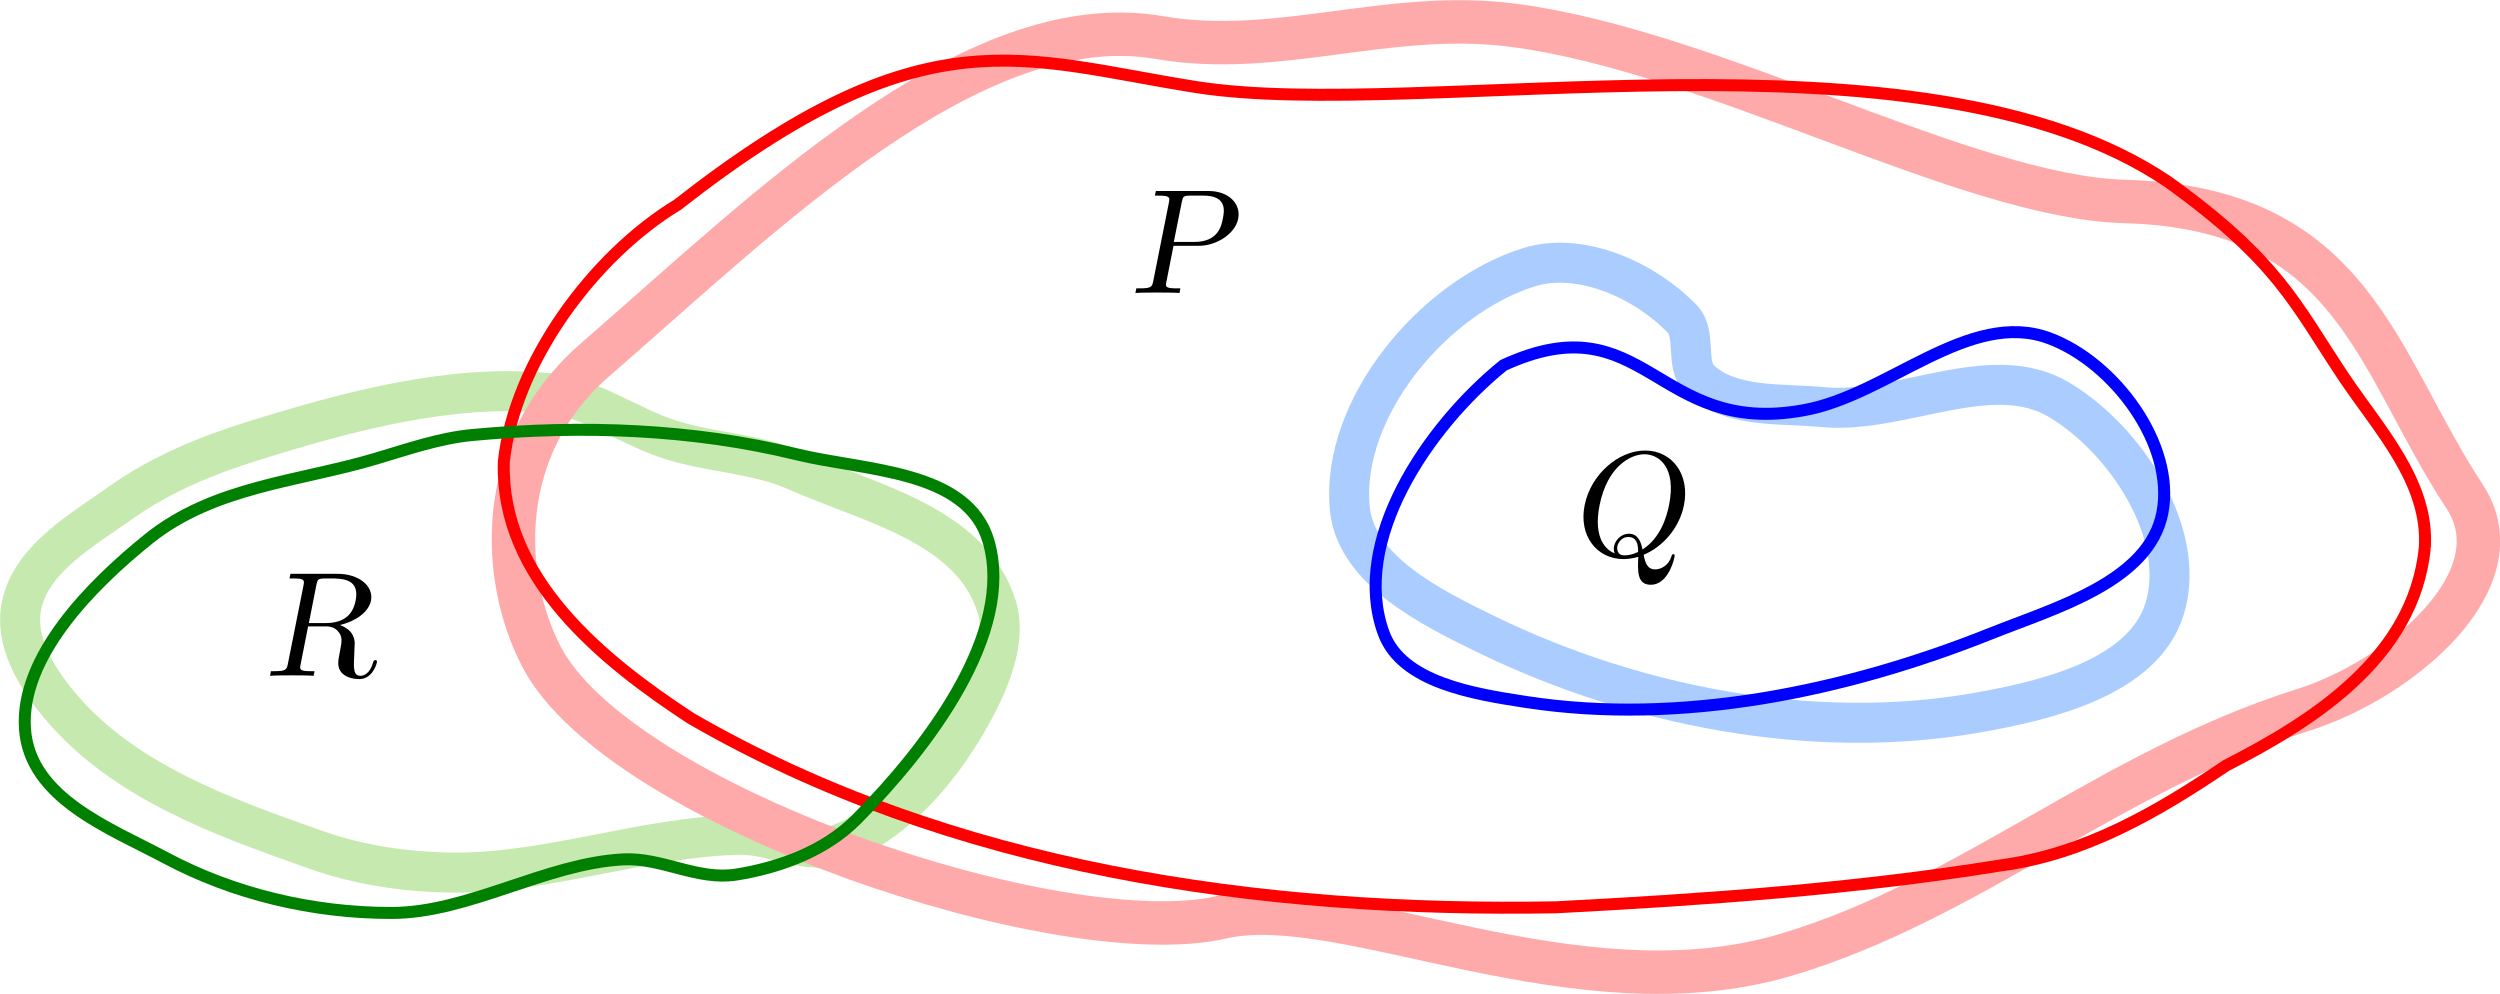
\includegraphics[scale=0.5]{../2020/floating-sets-1.png}}}
\qquad
\vcenter{\hbox{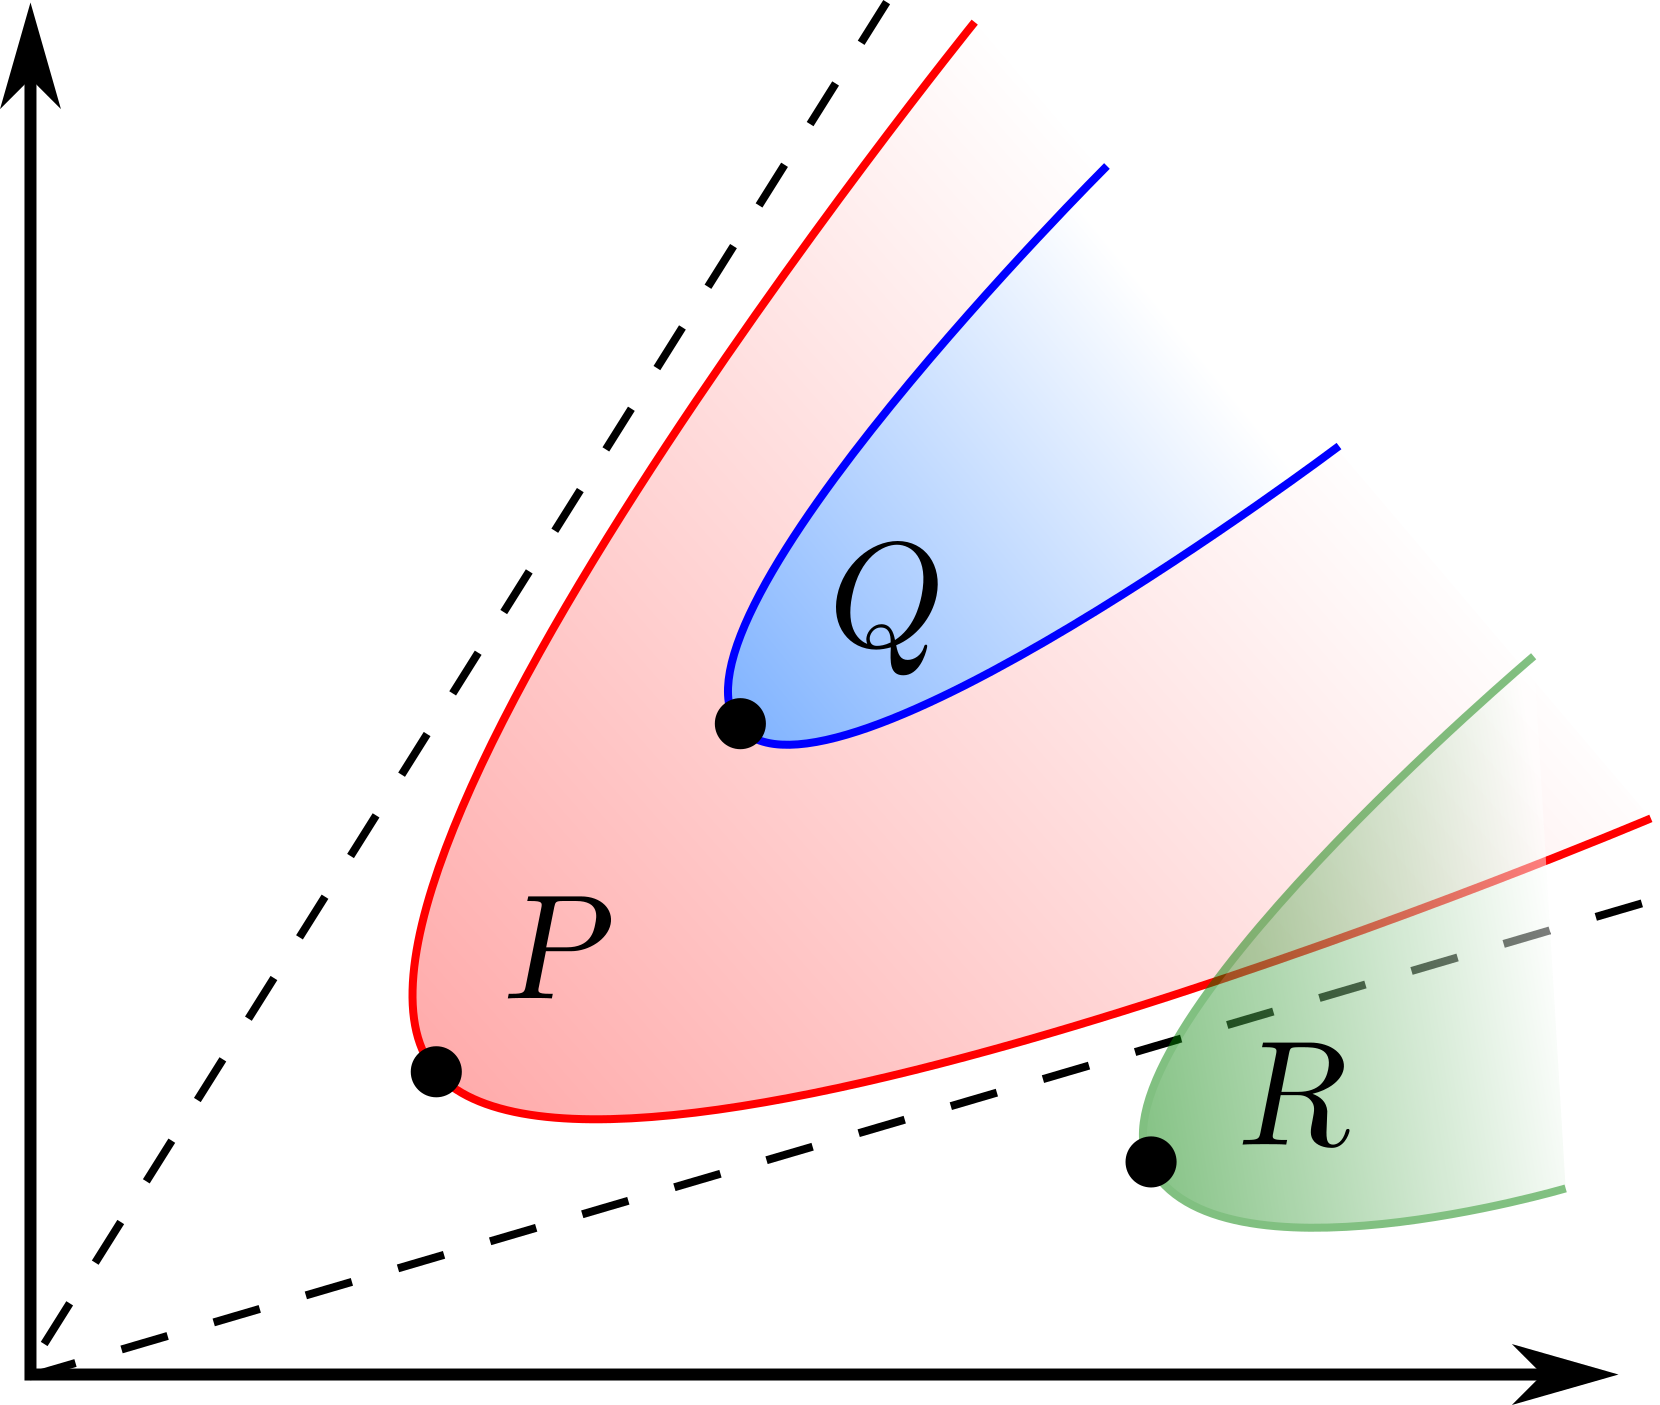
\includegraphics[scale=0.5]{../2020/floating-sets-2.png}}}
\end{equation}

%\begin{equation}
%\begin{tikzpicture}[overlay]
%% \draw  plot[smooth, tension=.9] coordinates {(-2,0) (0,1) (2,0) (0,-1)  (-2,0)};
%\draw (0,0) ellipse (3cm and 1cm);
%\end{tikzpicture}
%\bullet \mathrm{John}
%\end{equation}

\cc{Then how is the spatial model better than a syntactic representation (bunch of propositions)?
}{
	Then how is the spatial model better than a syntactic representation (bunch of propositions)?
}

\newtheorem{thm}{Definition}
\begin{thm}
	\cc{	\emp{Deep learning} consists of a \textbf{hierarchical} structure with many levels (hence ``deep'') where the structure is learned to fit data.  Such a learning algorithm must be \textbf{efficient}.
	}{
		\emp{Deep learning} consists of a \textbf{hierarchical} structure with many levels (hence ``deep'') where the structure is learned to fit data.  Such a learning algorithm must be \textbf{efficient}.
	}
\end{thm}
\cc{第二个条件加上去是因为,「经典」逻辑AI的 学习算法 也符合「深度」条件,但它不够效率。 
}{
	The second condition is added because the learning algorithm of "classical" logic AI also meets the "depth" condition, but it is not efficient enough.
}

\section*{References}
\cc{欢迎提问和讨论}{Questions, comments welcome} \smiley \\ \vspace*{0.4cm}
\printbibliography

\end{document} 
